\documentclass[a4paper,12pt]{article}

%----------------------- 宏包引入 -----------------------
\usepackage{ctex}       % 中文支持
\usepackage{graphicx}   % 图片支持
\usepackage{geometry}   % 页面布局
\usepackage{listings}   % 代码展示
\usepackage{xcolor}     % 颜色支持
\usepackage{hyperref}   % 超链接
\usepackage{amsmath}    % 数学公式
\usepackage{amssymb}    % 数学符号
\usepackage{booktabs}   % 专业表格
\usepackage{fancyhdr}   % 页眉页脚
\usepackage{lastpage}   % 引用最后一页
\usepackage{caption}    % 标题设置
\usepackage{subfigure}  % 子图支持
\usepackage{float}      % 强制图片位置
\usepackage{enumitem}   % 列表优化
\usepackage{tikz}       % 绘图工具
\usepackage{pgfplots}   % 画折线图
\usepackage{longtable}  % 长表格支持
\usepackage{array}      % 表格增强
\usepackage{multirow}   % 多行单元格
\usepackage{tabularx}   % 自动列宽
\usepackage{placeins}   % 控制浮动体
\pgfplotsset{width=10cm,compat=1.9}
\usetikzlibrary{shapes,arrows,positioning,automata,calc,arrows.meta}

%----------------------- 页面设置 -----------------------
\geometry{left=2.5cm,right=2.5cm,top=2.8cm,bottom=2.8cm}
\linespread{1.5} 
\setlength{\headheight}{14.5pt}

%----------------------- 解决排版问题 -----------------------
\renewcommand{\textfraction}{0.05}
\renewcommand{\topfraction}{0.95}
\renewcommand{\bottomfraction}{0.95}
\renewcommand{\floatpagefraction}{0.8}
\setcounter{topnumber}{3}
\setcounter{bottomnumber}{3}
\setcounter{totalnumber}{5}

%----------------------- 代码高亮设置 -----------------------
\definecolor{codegreen}{rgb}{0,0.6,0}
\definecolor{codegray}{rgb}{0.5,0.5,0.5}
\definecolor{codepurple}{rgb}{0.58,0,0.82}
\definecolor{backcolour}{rgb}{0.97,0.97,0.97}

\lstdefinestyle{mystyle}{
    backgroundcolor=\color{backcolour},   
    commentstyle=\color{codegreen}\itshape,
    keywordstyle=\color{blue}\bfseries,
    numberstyle=\tiny\color{codegray},
    stringstyle=\color{codepurple},
    basicstyle=\ttfamily\small, 
    breakatwhitespace=false,         
    breaklines=true,                 
    captionpos=b,                    
    keepspaces=true,                 
    numbers=left,                    
    numbersep=8pt,                  
    showspaces=false,                
    showstringspaces=false,
    showtabs=false,                  
    tabsize=4,
    frame=shadowbox,
    frameround=tttt,
    xleftmargin=2em,
    xrightmargin=1em,
    language=HTML
}
\lstset{style=mystyle}

%----------------------- 页眉页脚 -----------------------
\pagestyle{fancy}
\lhead{\kaishu 软件工程团队文档}
\chead{软件设计报告} 
\rhead{第15组} 
\lfoot{}
\cfoot{第 \thepage 页 \ / \ 共 \pageref{LastPage} 页}
\rfoot{}
\renewcommand{\headrulewidth}{0.4pt}

\begin{document}

%----------------------- 封面 -----------------------
\begin{titlepage}
  \begin{center}
    \vspace*{2cm}
    
\includegraphics[width=0.5\textwidth]{NKU.png} \\
    \vspace*{2cm}
    {\Huge \bfseries 软件工程团队报告} \\
    \vspace{1.5cm}
    {\Large \bfseries 团队作业2：软件设计报告} \\
    \vspace{3cm}

    \begin{tabular}{l l}
      \Large \textbf{团队组号：} & \Large 15                                      \\
      \Large \textbf{团队成员：} & \Large 杨雨杭、刘轩麟、尹浩燃、张启鑫、王增哲                     \\
      \Large \textbf{学号：}   & \Large 2310700、2312289、2313547、2313411、2310708 \\
      \Large \textbf{指导教师：} & \Large 徐思涵                                     \\
    \end{tabular}

    \vfill
    {\Large \today}
  \end{center}
\end{titlepage}

\newpage
\tableofcontents
\newpage

%----------------------- 正文开始 -----------------------

\section{一、系统总体设计}

\subsection{1. 项目背景与目标}
随着南开大学推理协会社团规模的日益扩大，传统的基于人工登记的剧本/书籍借阅、QQ群报名活动、以及零散的线下解谜互动已难以满足高效运营的需求。物资流转不透明、数据统计繁杂、社员活跃度缺乏直观反馈成为制约社团发展的痛点。本项目旨在利用微信开发者工具，构建一个集“推理、竞技、社交、管理”于一体的数字化平台，通过游戏化的机制增强社员粘性。

本系统旨在构建一个全方位的社团数字化管理闭环。其核心业务范围涵盖以下13个模块：
\begin{itemize}
  \item \textbf{日常互动}：每日谜题解答与解析、Dud关键词自动回复系统。
  \item \textbf{物资管理}：剧本杀与书籍借阅流转、后台物资库存清点系统。
  \item \textbf{激励体系}：动态更新的积分排行榜、独立逻辑的积分兑换商城、个人电子侦探名片。
  \item \textbf{活动与互助}：具备截止时间逻辑的活动报名系统、涉及积分悬赏的事件委托系统。
  \item \textbf{基础支撑}：账号注册与登录、系统设置、权限控制和通知偏好等常规小程序功能。
\end{itemize}

\subsection{2. 系统功能概述}
系统面向未登录用户（游客）、普通用户（侦探）与管理员（社团管理层）三类角色：未登录用户仅浏览公开内容；普通用户主要完成答题、报名、借阅、兑换、发帖和个人信息维护；管理员在继承普通用户能力的基础上，负责谜题、规则、库存、活动、借阅状态、反馈信息和官方委托的维护。

系统核心用例可分为日常互动、积分激励、活动互助、物资管理和后台维护五类。各用例之间以“微信授权登录”为权限入口，以“积分账户”和“库存管理”为共享业务基础。

\subsection{3. 系统总体架构设计}
NK推协侦探管理系统是一款面向高校推理协会社团运营场景的微信小程序，
系统涵盖每日谜题竞猜、积分体系、排行榜、活动报名、物资借阅、
积分商城兑换、事件委托、Dud关键词对话、推荐内容发布、反馈系统以及后台管理等模块。

系统整体采用”客户端-服务器 + Serverless 云原生”混合架构，
前端基于微信小程序实现，后端依托微信云开发 CloudBase。

\subsubsection{总体架构风格}

\begin{center}
  \begin{tikzpicture}[
    scale=0.85,
    transform shape,
    node distance=1.2cm,
    box/.style={
        rectangle,
        draw,
        rounded corners,
        minimum width=3.2cm,
        minimum height=0.9cm,
        align=center
      },
    arrow/.style={-{Latex[length=2.5mm]},thick}
    ]

    \node[box] (client) {微信小程序客户端\\Pages / Components / Services};
    \node[box,below=of client] (gateway) {wx.cloud.callFunction + HTTPS};
    \node[box,below left=1.5cm and 2.5cm of gateway] (faas) {Cloud Functions\\Serverless FaaS};
    \node[box,below=of gateway] (db) {Cloud Database\\NoSQL BaaS};
    \node[box,below right=1.5cm and 2.5cm of gateway] (storage) {Cloud Storage\\COS};

    \draw[arrow] (client)--(gateway);
    \draw[arrow] (gateway)--(faas);
    \draw[arrow] (gateway)--(db);
    \draw[arrow] (gateway)--(storage);

  \end{tikzpicture}
\end{center}

\subsubsection{架构风格对照表}

\begin{longtable}{p{4cm} p{5cm} p{5cm}}
  \toprule
  架构风格         & 系统体现                          & 作用       \\ \midrule
  客户端-服务器架构    & 微信小程序 + 腾讯云                   & 实现前后端分离  \\
  Serverless架构 & 云函数 + 云数据库                    & 降低运维成本   \\
  分层架构         & 表现层/服务层/工具层                   & 提升可维护性   \\
  领域模块化        & puzzle / ranking / borrow 等模块 & 降低耦合度    \\
  RBAC权限控制     & user/admin 角色体系               & 强化安全性    \\
  事件驱动         & 排行榜定时快照                       & 提升异步处理能力 \\
  \bottomrule
\end{longtable}

\subsubsection{系统物理部署架构}

\begin{center}
  \resizebox{\textwidth}{!}{
    \begin{tikzpicture}[
      box/.style={rectangle,draw,rounded corners,align=center},
      arrow/.style={-{Latex[length=3mm]},thick}
      ]

      \node[box,minimum width=6cm,minimum height=2cm] (client) {
        微信小程序客户端\\
        首页 / 排行榜 / 我的 / 每日谜题\\
        分包页面 + Components
      };

      \node[box,below=2cm of client,minimum width=10cm,minimum height=6cm] (cloud) {
        腾讯云 CloudBase
      };

      \node[box,inner sep=5pt] at ([yshift=1.5cm]cloud.center) (faas) {
        云函数层\\
        user / puzzle / ranking / borrow / exchange / admin ...
      };

      \node[box,inner sep=5pt] at (cloud.center) (database) {
        云数据库层\\
        users / puzzles / points\_log / inventory\_items / ranking\_snapshots ...
      };

      \node[box,inner sep=5pt] at ([yshift=-1.5cm]cloud.center) (storage) {
        云存储层\\
        头像 / 海报 / 推荐图片
      };

      \draw[arrow] (client)--node[right]{wx.cloud.callFunction()} (cloud);

    \end{tikzpicture}
  }
\end{center}

\subsubsection{客户端架构设计}

\textbf{客户端四层结构：}

\begin{center}
  \begin{tikzpicture}[
    layer/.style={rectangle,draw,minimum width=10cm,minimum height=1.2cm,align=center,font=\small},
    arrow/.style={-{Latex[length=2mm]},thick}
    ]

    \node[layer] (presentation) {
      表现层 — Pages + Components
    };

    \node[layer,below=0.2cm of presentation] (service) {
      业务服务层 — PuzzleService / RankingService / BorrowService / ActivityService ...
    };

    \node[layer,below=0.2cm of service] (utils) {
      工具层 — request / auth / storage / validate / format
    };

    \node[layer,below=0.2cm of utils] (config) {
      配置层 — config/index.js
    };

    \draw[arrow] (presentation)--(service);
    \draw[arrow] (service)--(utils);
    \draw[arrow] (utils)--(config);

  \end{tikzpicture}
\end{center}

\textbf{客户端页面分包策略：}

\begin{longtable}{p{3cm} p{10.5cm}}
  \toprule
  页面类型 & 内容                                                       \\ \midrule
  主包页面 & 首页、排行榜、每日谜题、个人中心                                         \\
  分包页面 & admin、activity、borrow、exchange、commission、dud、feedback 等 \\
  优化策略 & lazyCodeLoading + 按需加载 + 组件复用                            \\
  \bottomrule
\end{longtable}

\textbf{客户端通信模型：}

\begin{center}
  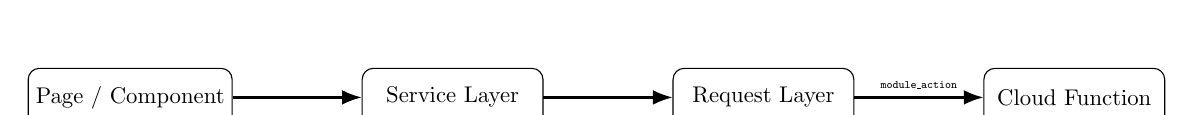
\begin{tikzpicture}[
    scale=0.82,
    transform shape,
    box/.style={
        rectangle,
        draw,
        rounded corners,
        minimum width=2.8cm,
        minimum height=0.9cm,
        align=center
      },
    arrow/.style={-{Latex[length=2.5mm]},thick}
    ]

    \node[box] (page) {Page / Component};
    \node[box,right=2cm of page] (service) {Service Layer};
    \node[box,right=2cm of service] (request) {Request Layer};
    \node[box,right=2cm of request] (cloud) {Cloud Function};

    \draw[arrow] (page)--(service);
    \draw[arrow] (service)--(request);
    \draw[arrow] (request)--node[above, font=\tiny\ttfamily]{module\_action} (cloud);

  \end{tikzpicture}
\end{center}

\subsubsection{服务端架构设计}

\textbf{云函数 Action 路由机制：}

\begin{center}
  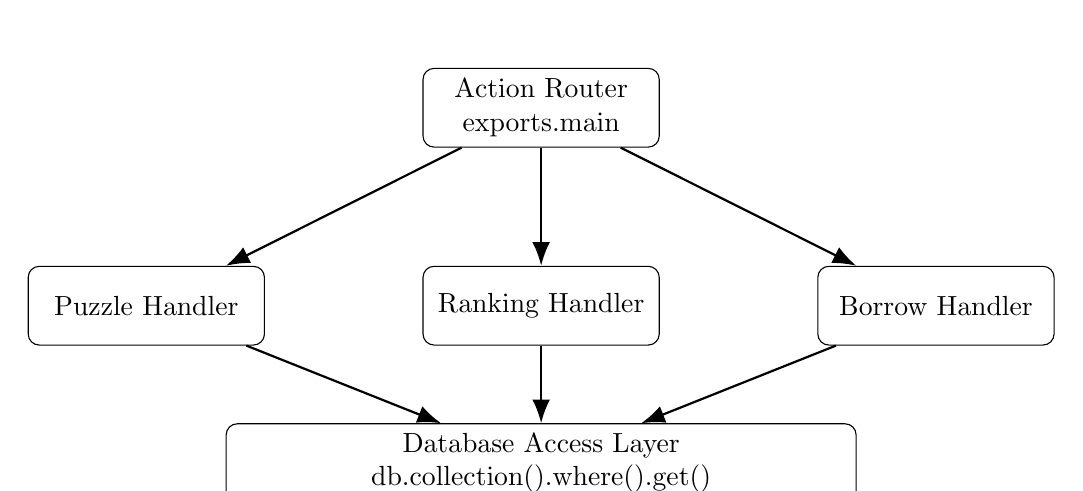
\begin{tikzpicture}[
    box/.style={rectangle,draw,rounded corners,minimum width=3cm,minimum height=1cm,align=center},
    arrow/.style={-{Latex[length=3mm]},thick}
    ]

    \node[box] (router) {Action Router\\exports.main};

    \node[box,below left=1.5cm and 2cm of router] (handler1) {Puzzle Handler};
    \node[box,below=1.5cm of router] (handler2) {Ranking Handler};
    \node[box,below right=1.5cm and 2cm of router] (handler3) {Borrow Handler};

    \node[box,below=3.5cm of router,minimum width=8cm] (db) {
      Database Access Layer\\
      db.collection().where().get()
    };

    \draw[arrow] (router)--(handler1);
    \draw[arrow] (router)--(handler2);
    \draw[arrow] (router)--(handler3);

    \draw[arrow] (handler1)--(db);
    \draw[arrow] (handler2)--(db);
    \draw[arrow] (handler3)--(db);

  \end{tikzpicture}
\end{center}

\textbf{云函数目录：}

\begin{verbatim}
cloudfunctions/
├── user/           ├── activity/      ├── commission/
├── puzzle/         ├── borrow/        ├── dud/
├── ranking/        ├── exchange/      ├── profile/
├── points/         ├── feedback/      ├── recommendation/
├── admin/          └── init_db/
\end{verbatim}

\textbf{权限控制体系：}

\begin{center}
  \begin{tikzpicture}[
    box/.style={rectangle,draw,rounded corners,minimum width=4cm,minimum height=1cm,align=center},
    arrow/.style={-{Latex[length=3mm]},thick}
    ]

    \node[box] (login) {微信登录\\wx.login()};
    \node[box,below=1.2cm of login] (openid) {获取 OPENID};
    \node[box,below left=1.5cm and 2.5cm of openid] (user) {普通用户\\答题/报名/借阅};
    \node[box,below right=1.5cm and 2.5cm of openid] (admin) {管理员\\系统管理/日志};

    \draw[arrow] (login)--(openid);
    \draw[arrow] (openid)--(user);
    \draw[arrow] (openid)--(admin);

  \end{tikzpicture}
\end{center}

\subsubsection{数据架构设计}

\textbf{积分系统数据模型：}

\begin{center}
  \begin{tikzpicture}[
      box/.style={rectangle,draw,rounded corners,minimum width=5cm,minimum height=0.8cm,align=left,font=\small}
    ]

    \node[box] (t) {total\_points：累计积分};
    \node[box,below=0.2cm of t] (a) {available\_points：可用积分};
    \node[box,below=0.2cm of a] (f) {frozen\_points：冻结积分};
    \node[box,below=0.2cm of f] (u) {used\_points：已消耗积分};

  \end{tikzpicture}
\end{center}

\vspace{0.3cm}

\[
  available = total - frozen - used
\]

\textbf{数据库安全模型：}

\begin{longtable}{p{4cm} p{7cm} p{3cm}}
  \toprule
  安全级别  & 规则                        & 典型集合                 \\ \midrule
  公开读取  & read=true                 & puzzles / activities \\
  仅本人读取 & doc.openid == auth.openid & users / feedback     \\
  关联读取  & 关联用户身份校验                  & point\_accounts      \\
  禁止读取  & read=false                & admin\_logs          \\
  \bottomrule
\end{longtable}

\textbf{系统质量属性：}

\begin{longtable}{p{4cm} p{10cm}}
  \toprule
  质量属性 & 设计措施                      \\ \midrule
  安全性  & OpenID鉴权 + 数据库安全规则 + 审计日志 \\
  可靠性  & 指数退避重试 + 幂等机制 + 请求去重      \\
  性能   & 分包加载 + 缓存 + 原子更新          \\
  可维护性 & 分层架构 + 配置集中化 + init\_db迁移 \\
  可扩展性 & 新模块可独立扩展云函数与Service       \\
  可测试性 & 服务层与视图层解耦                 \\
  \bottomrule
\end{longtable}
系统采用客户端-服务器与Serverless融合架构，
在保证低运维成本的同时，实现了良好的扩展性、可靠性与可维护性。
通过分层架构、动作路由、RBAC权限控制以及数据库安全规则，
形成了一套适用于高校社团管理场景的完整云原生解决方案。

\subsection{4. 技术选型说明}

本系统的技术选型围绕“快速交付、低成本运维、与微信生态深度融合”三大目标展开。以下分层面阐述选型决策及其理由。

\textbf{客户端运行时：微信小程序原生框架。} 微信小程序无需用户下载安装，依托微信庞大的用户基数和社交传播链条，天然适合面向社团成员的应用场景。其原生框架提供 WXML 声明式模板语言（类似 HTML）和 WXSS 样式语言（兼容 CSS 大部分特性），开发者可以基于传统的 Web 前端技能快速上手。同时，小程序原生 API 提供了微信登录、用户信息获取、位置服务等基础设施，无需自行搭建认证体系。

\textbf{前端开发语言：JavaScript（ES6+）。} 选择 JavaScript 而非 TypeScript 的原因在于微信小程序对原生 JS 的支持最为成熟稳定，且项目规模适中，JS 的动态特性和简练语法反而有助于快速迭代。前端工程中充分利用了 ES6 的模块化机制（\texttt{require/module.exports}）、箭头函数、解构赋值与 async/await 异步语法，代码组织清晰，可读性强。

\textbf{服务端运行时：Node.js 云函数。} 微信云开发的云函数本质上是部署在腾讯云上的 Node.js 无服务器函数。选择这一方案而非自建服务器或传统云主机，理由有三：其一，免运维——无需管理服务器实例、操作系统补丁或负载均衡；其二，按量计费——社团级应用的请求量较低，无服务器架构可大幅降低成本；其三，与云数据库的原生集成——云函数通过 \texttt{wx-server-sdk} 可直接访问云数据库、云存储和云调用，无需配置额外的网络通路或鉴权逻辑。

\textbf{数据库：微信云数据库（文档型 NoSQL）。} 微信云数据库是一种面向 JSON 文档的 NoSQL 数据库，在数据模型上与 MongoDB 类似。选择 NoSQL 而非关系型数据库的核心考量：社团应用的数据结构处于频繁迭代状态（如活动报名字段、借阅状态流转规则会在运营过程中调整），NoSQL 的无模式（schemaless）特性允许灵活修改文档字段而无需执行 DDL 操作；同时，云数据库与云函数共享同一腾讯云环境，数据读写延迟低，且安全规则引擎支持基于文档字段的细粒度权限控制。

\textbf{认证方案：微信 OpenID。} 系统不自行维护用户名/密码体系，而是基于微信登录获取用户的唯一 OpenID 标识。云函数通过 \texttt{cloud.\allowbreak getWXContext().\allowbreak OPENID} 获取调用者的 OpenID，以此关联 \texttt{users} 集合中的用户文档。这一设计消除了密码存储与验证的安全风险，也简化了用户端的注册流程。

\textbf{其他工具与中间件。} 前端请求层实现了超时控制（默认10秒）、自动重试（指数退避）与统一错误码映射，以应对移动网络的不稳定性。本地存储模块（\texttt{storage.js}）为排行榜、用户信息、推荐内容等数据提供带过期时间的缓存策略，减少不必要的云函数调用。此外，项目无需引入第三方中间件或外部服务，全部能力由微信云开发生态原生提供，技术栈简洁统一。

各层面的技术选型汇总如下：

\begin{table}[H]
  \centering
  \caption{技术选型汇总}
  \label{tab:tech-stack}
  \scriptsize
  \resizebox{\textwidth}{!}{\begin{tabular}{p{2.5cm} p{3.2cm} p{3cm} p{5cm}}
      \toprule
      \textbf{层面} & \textbf{技术选择}   & \textbf{版本/规格} & \textbf{选型核心理由}        \\
      \midrule
      客户端运行时      & 微信小程序原生框架       & 基础库 3.16.0     & 免安装、微信生态融合、原生API丰富     \\
      \midrule
      前端语言        & JavaScript ES6+ & ES6 模块化        & 小程序原生支持最成熟，动态特性利于迭代    \\
      \midrule
      视图模板        & WXML + WXSS     & 小程序标记/样式语言     & 声明式UI，类HTML/CSS上手快     \\
      \midrule
      服务端运行时      & Node.js 云函数     & wx-server-sdk  & 无服务器免运维，按量计费，与云数据库原生集成 \\
      \midrule
      数据库         & 微信云数据库          & 文档型 NoSQL      & 无模式灵活迭代，安全规则引擎细粒度权限控制  \\
      \midrule
      认证方案        & 微信 OpenID       & OAuth 2.0      & 无需维护密码体系，服务端注入不可伪造     \\
      \midrule
      开发工具        & 微信开发者工具         & 稳定版            & 一键预览/调试/上传，云开发控制台集成    \\
      \bottomrule
    \end{tabular}}
\end{table}

\section{二、详细设计}

\subsection{1. 模块划分与模块功能设计}

本系统在前后端均按业务子域进行了明确的模块划分。前端侧划分为页面模块、业务服务模块、公共组件模块和工具模块四个层次；后端侧则将一个业务子域映射为一个云函数模块，每个云函数内部通过 \texttt{action} 参数实现子操作的动态路由。

\textbf{用户与认证模块（\texttt{user} 云函数 + \texttt{auth.js} 工具层）。} 该模块是系统的权限入口。前端 \texttt{auth.js} 负责微信登录流程、Token 管理与本地用户信息缓存；后端 \texttt{user} 云函数处理 OpenID 解析、用户文档的首次创建与登录时更新、个人信息维护，并自动同步 \texttt{profile\_cards} 名片集合。

\textbf{每日谜题模块（\texttt{puzzle} 云函数 + \texttt{pages/puzzle} 页面）。} 负责每日推理谜题的发布、展示、答题与历史查询。核心逻辑包括：按日期匹配当天已发布的谜题，支持四个选项的标准化建模（\texttt{puzzle\_options} 集合），答题采用稳定 \_id 幂等写入防止重复答题与双倍加分，答对后通过 \texttt{db.command.inc} 原子递增用户积分并写入积分流水。每人每日限答一次。

\textbf{积分管理模块（\texttt{points} 云函数 + \texttt{pages/points} 页面）。} 积分为系统的核心激励资源，拆分为四个维度的账户：总积分（\texttt{total\_points}，用于排行榜排名）、可兑换积分（\texttt{available\_points}，用于商城和委托）、冻结积分（\texttt{frozen\_points}，用于委托发布时锁定）和已用积分（\texttt{used\_points}）。积分账户在 \texttt{point\_accounts} 和 \texttt{users} 两处双写以支持不同的查询场景。每次积分变动均写入 \texttt{points\_log} 流水，可追溯完整的积分来源与去向。

\textbf{排行榜模块（\texttt{ranking} 云函数 + \texttt{pages/ranking} 页面）。} 提供前三名展示与完整榜单查询，支持同分并列排名。排行榜数据定期生成快照写入 \texttt{ranking\_snapshots} 集合，前端配合60秒本地缓存以降低云函数调用频率。排行榜用户项可点击跳转至对应的个人侦探名片。

\textbf{活动报名模块（\texttt{activity} 云函数 + \texttt{pages/activity} 页面）。} 管理活动的发布、浏览、报名和取消报名。后端校验重复报名、容量上限与取消截止时间。活动状态包括“报名中”“已满”“已结束”“已取消”四种流转。报名记录写入 \texttt{activity\_registrations} 集合并关联用户 ID。

\textbf{物资借阅模块（\texttt{borrow} 云函数 + \texttt{pages/borrow} 页面）。} 统一管理书籍、剧本杀和物资的库存与流转。库存数据集中在 \texttt{inventory\_items} 集合，通过 \texttt{item\_type} 字段区分物资类型（book、script、supplies）。借阅状态流转包括“在库→借用中→已借出→已归还/已取消”四个阶段，每次状态变更通过条件更新（\texttt{where\{status:\allowbreak\ oldStatus\}} 后 \texttt{update}）确保并发安全。借阅申请失败时自动回滚物资状态。

\textbf{积分兑换模块（\texttt{exchange} 云函数 + \texttt{pages/exchange} 页面）。} 提供积分商城功能，用户可使用可兑换积分兑换商品。兑换时需按商品所需积分扣减用户 \texttt{available\_points} 并写入\\
\texttt{exchange\_records} 记录。兑换商品与借阅物资共享 \texttt{inventory\_items} 集合以统一库存管理。

\textbf{事件委托模块（\texttt{commission} 云函数 + \texttt{pages/commission} 页面）。} 实现积分悬赏的任务发布与领取机制。发布者发布委托时系统原子冻结其可兑换积分；领取者完成委托后发布者分配奖励积分，系统将冻结积分解冻并转入领取者账户。采用严格的条件原子更新防止双重分配：领取记录的 \texttt{completed→rewarded} 流转和委托的 \texttt{remaining\_reward\allowbreak\ >= points} 校验均在单条命令中完成。管理员的官方委托由系统提供积分奖励而非发布者个人积分。

\textbf{Dud 关键词回复模块（\texttt{dud} 云函数 + \texttt{pages/dud} 页面）。} 实现简单的关键词匹配自动回复。管理员在后台维护关键词规则（包括精确匹配和模糊匹配两种模式），用户发送消息时系统遍历规则集合并返回最先匹配到的回复文本。前端提供聊天界面，后台可管理规则的优先级和启用状态。

\textbf{反馈留言模块（\texttt{feedback} 云函数 + \texttt{pages/feedback} 页面）。} 用户可通过此模块提交对社团或系统的反馈建议，支持匿名选项。管理员在后台浏览所有反馈并填写处理备注。反馈数据按用户 ID 关联，用户仅可查看自己提交的反馈记录。

\textbf{推荐内容模块（\texttt{recommendation} 云函数 + \texttt{pages/recommendation} 页面）。} 管理员可在后台发布推荐内容（如社团资讯、优秀推理作品推荐等），前端首页展示推荐摘要，用户可点击进入详情页。

\textbf{个人名片模块（\texttt{profile} 云函数 + \texttt{pages/profile} 页面）。} 为用户提供电子侦探名片功能，展示昵称、校区、年级、专业、兴趣标签、个人简介及喜爱的推理作品。名片可设置为公开或私有，排行榜等处可跳转查看其他用户的名片。名片数据存储在独立的 \texttt{profile\_cards} 集合中。

\textbf{管理后台模块（\texttt{admin} 云函数 + \texttt{pages/admin} 页面）。} 为社团管理层提供一站式后台管理入口。基于用户文档中的 \texttt{role=admin} 字段进行权限校验。提供数据概览统计以及谜题发布、活动管理、库存维护、兑换商品管理、推荐内容上下架、Dud 规则编辑、反馈处理、系统设置等各项管理功能。关键管理操作写入 \texttt{admin\_logs} 记录。

\textbf{模块间调用关系。} 各模块通过积分账户实现横向关联：谜题答题、委托奖励等模块向积分模块写入流水并更新账户余额；积分余额又是排行榜的数据源和商城兑换的扣减依据。借阅、兑换模块共享 \texttt{inventory\_items} 作为统一库存。用户模块提供的用户标识和角色信息是所有其他模块进行身份认证和权限判断的基础。模块间不存在直接的云函数调用，数据耦合通过共享数据库集合实现，保持了各模块的独立部署和独立演化能力。

各模块的组成部分与职责汇总如下：

\begin{table}[H]
  \centering
  \caption{系统模块划分一览}
  \label{tab:modules}
  \scriptsize
  \resizebox{\textwidth}{!}{\begin{tabular}{p{2.2cm} p{2.8cm} p{3.2cm} p{5.4cm}}
      \toprule
      \textbf{模块} & \textbf{后端云函数}          & \textbf{前端页面/组件}              & \textbf{核心职责}                        \\
      \midrule
      用户与认证       & \texttt{user}           & \texttt{auth.js}（工具层）         & 微信登录、OpenID解析、用户自动注册/更新、个人资料维护、管理员晋升 \\
      \midrule
      每日谜题        & \texttt{puzzle}         & \texttt{pages/puzzle}         & 每日谜题发布与展示、选项建模、答题幂等防重、答对加分           \\
      \midrule
      积分管理        & \texttt{points}         & \texttt{pages/points}         & 四维积分账户（总额/可用/冻结/已用）、流水记录、原子增减        \\
      \midrule
      排行榜         & \texttt{ranking}        & \texttt{pages/ranking}        & 前三名展示、完整榜单、同分并列、排行榜快照缓存              \\
      \midrule
      活动报名        & \texttt{activity}       & \texttt{pages/activity}       & 活动发布与管理、报名/取消、容量校验、截止时间控制            \\
      \midrule
      物资借阅        & \texttt{borrow}         & \texttt{pages/borrow}         & 统一库存管理、借阅状态流转、条件原子更新、失败自动回滚          \\
      \midrule
      积分兑换        & \texttt{exchange}       & \texttt{pages/exchange}       & 积分商城、库存/积分双扣减、兑换记录追踪                 \\
      \midrule
      事件委托        & \texttt{commission}     & \texttt{pages/commission}     & 积分悬赏发布与领取、冻结-分配-解冻机制、双重原子校验          \\
      \midrule
      Dud 回复      & \texttt{dud}            & \texttt{pages/dud}            & 关键词匹配（精确/模糊）、优先级排序、聊天界面              \\
      \midrule
      反馈留言        & \texttt{feedback}       & \texttt{pages/feedback}       & 用户反馈提交（支持匿名）、管理员处理备注                 \\
      \midrule
      推荐内容        & \texttt{recommendation} & \texttt{pages/recommendation} & 推荐内容发布与上下架、首页摘要展示                    \\
      \midrule
      个人名片        & \texttt{profile}        & \texttt{pages/profile}        & 电子侦探名片、公开/私有设置、跨页面名片查看               \\
      \midrule
      管理后台        & \texttt{admin}          & \texttt{pages/admin}          & 全局数据概览、全业务域后台管理、权限校验、操作审计            \\
      \bottomrule
    \end{tabular}}
\end{table}

\subsection{2. 核心业务流程设计}

本系统的核心业务流程围绕用户登录、每日谜题答题、物资借阅流转、事件委托生命周期和积分兑换展开。以下通过流程图结合文字说明，逐一描述各流程的关键步骤与设计决策。

\subsubsection*{2.1 用户授权登录流程}

用户首次打开小程序时，客户端调用 \texttt{wx.login()} 获取微信临时凭证，随后调用 \texttt{user} 云函数的 \texttt{login} action。云函数通过 \texttt{cloud.\allowbreak getWXContext().\allowbreak OPENID} 获取用户唯一标识，查询 \texttt{users} 集合：若用户不存在，则自动创建用户文档并同步生成 \texttt{profile\_cards} 个人名片；若用户已存在，则更新最后登录时间并补全缺失字段。登录成功后，客户端将用户信息缓存在 \texttt{app.globalData} 和本地存储中，后续页面可直接读取而无需重复调用云函数。

\begin{figure}[H]
  \centering
  \resizebox{0.68\textwidth}{!}{
    \begin{tikzpicture}[
        box/.style={rectangle, draw=black, rounded corners=3pt, minimum width=2.2cm, minimum height=0.7cm, font=\footnotesize, align=center, fill=blue!5},
        decision/.style={diamond, draw=black, aspect=1.8, minimum width=1.8cm, minimum height=0.8cm, font=\footnotesize, align=center, fill=yellow!8},
        startend/.style={rectangle, draw=black, rounded corners=12pt, minimum width=2cm, minimum height=0.7cm, font=\footnotesize, align=center, fill=green!10},
        arrow/.style={>=stealth, ->, thick},
        label/.style={font=\scriptsize\itshape},
      ]
      \node [startend] (start) {用户打开小程序};
      \node [box, below=0.8cm of start] (wxlogin) {wx.login() 获取临时凭证};
      \node [box, below=0.7cm of wxlogin] (calluser) {调用 user 云函数\\\texttt{action: login}};
      \node [box, below=0.7cm of calluser] (getopenid) {cloud.getWXContext()\\获取 OpenID};
      \node [box, below=0.7cm of getopenid] (queryuser) {查询 users 集合\\(where: \{openid\})};
      \node [decision, below=0.9cm of queryuser] (exists) {用户存在?};
      \node [box, right=2.5cm of exists] (create) {创建用户文档\\+ profile\_cards\\+ 初始化积分账户};
      \node [box, below=0.9cm of exists] (update) {更新 last\_login\_at\\补全缺失字段};
      \node [box, below=0.7cm of update] (cache) {缓存至 app.globalData\\与本地存储};
      \node [startend, below=0.8cm of cache] (done) {登录完成};
      \draw [arrow] (start) -- (wxlogin);
      \draw [arrow] (wxlogin) -- (calluser);
      \draw [arrow] (calluser) -- (getopenid);
      \draw [arrow] (getopenid) -- (queryuser);
      \draw [arrow] (queryuser) -- (exists);
      \draw [arrow] (exists) -- node [label, above] {否} (create);
      \draw [arrow] (create) |- (cache);
      \draw [arrow] (exists) -- node [label, right] {是} (update);
      \draw [arrow] (update) -- (cache);
      \draw [arrow] (cache) -- (done);
    \end{tikzpicture}
  }
  \caption{用户授权登录流程}
  \label{fig:flow-login}
\end{figure}

\subsubsection*{2.2 每日谜题答题流程}

用户进入谜题页面后，前端按日期匹配当天已发布谜题，同时查询答题记录判断是否已作答。答题时采用稳定 \texttt{\_id} 幂等写入（格式为\\
\texttt{pa\_\{userId\}\_\{puzzleId\}\_\{date\}}），并发重复提交因 \texttt{\_id} 唯一性约束被数据库拒绝后自动返回已有结果。答对时通过 \texttt{db.command.inc} 原子递增积分并写入流水。

\begin{figure}[H]
  \centering
  \resizebox{0.70\textwidth}{!}{
    \begin{tikzpicture}[
        box/.style={rectangle, draw=black, rounded corners=3pt, minimum width=2.2cm, minimum height=0.7cm, font=\footnotesize, align=center, fill=blue!5},
        decision/.style={diamond, draw=black, aspect=1.8, minimum width=1.8cm, minimum height=0.8cm, font=\footnotesize, align=center, fill=yellow!8},
        startend/.style={rectangle, draw=black, rounded corners=12pt, minimum width=2cm, minimum height=0.7cm, font=\footnotesize, align=center, fill=green!10},
        db/.style={rectangle, draw=black!50, dashed, minimum width=2.8cm, minimum height=0.6cm, font=\footnotesize\ttfamily, align=center, fill=gray!5},
        arrow/.style={>=stealth, ->, thick},
        label/.style={font=\scriptsize\itshape},
      ]
      \node [startend] (start) {进入谜题页面};
      \node [box, below=0.7cm of start] (getpuzzle) {puzzle\_getTodayPuzzle\\按日期匹配谜题};
      \node [db, below=0.6cm of getpuzzle, xshift=-2.5cm] (db1) {puzzles};
      \node [db, below=0.6cm of getpuzzle] (db2) {puzzle\_options};
      \node [db, below=0.6cm of getpuzzle, xshift=2.5cm] (db3) {puzzle\_answers};
      \node [box, below=0.8cm of db2] (display) {展示题目与选项\\标注已答状态};
      \node [decision, below=0.8cm of display] (answered) {用户选择\\答案提交};
      \node [box, right=3cm of answered] (idem) {幂等检查：稳定\_id\\写入 puzzle\_answers};
      \node [decision, below=3.5cm of answered] (conflict) {\_id 冲突?};
      \node [decision, below=0.8cm of idem] (correct) {答对?};
      \node [box, below=0.7cm of correct] (addpts) {db.command.inc\\原子递增 total\_points\\和 available\_points};
      \node [box, left=2.5cm of addpts] (writelog) {写入 points\_log\\积分流水};
      \node [box, right=2cm of correct] (wrong) {返回答题结果\\(答错)};
      \node [box, right=2cm of conflict] (returndup) {返回已有记录\\(幂等返回)};
      \node [startend, below=0.8cm of addpts] (done) {答题完成};
      \draw [arrow] (start) -- (getpuzzle);
      \draw [arrow, dashed, draw=black!50] (getpuzzle) -- (db1);
      \draw [arrow, dashed, draw=black!50] (getpuzzle) -- (db2);
      \draw [arrow, dashed, draw=black!50] (getpuzzle) -- (db3);
      \draw [arrow] (getpuzzle) -- (display);
      \draw [arrow] (display) -- (answered);
      \draw [arrow] (answered) -- node [label, above] {点击提交} (idem);
      \draw [arrow] (idem) -- (conflict);
      \draw [arrow] (conflict) -- node [label, right] {是} (returndup);
      \draw [arrow] (conflict) -- node [label, left] {否} (correct);
      \draw [arrow] (correct) -- node [label, right] {是} (addpts);
      \draw [arrow] (correct) -- node [label, above] {否} (wrong);
      \draw [arrow] (addpts) -- (writelog);
      \draw [arrow] (writelog) |- (done);
      \draw [arrow] (addpts) -- (done);
    \end{tikzpicture}
  }
  \caption{每日谜题答题流程}
  \label{fig:flow-puzzle}
\end{figure}

\subsubsection*{2.3 物资借阅流转流程}

借阅流程的核心是库存状态的原子流转与失败回滚。申请时以条件更新（\texttt{where\{status:\allowbreak\ 'available'\}}）将物资从”在库”转为”传递中”，若条件不满足（已被他人借出）则拒绝请求。后续步骤失败时自动回滚物资状态并标记申请为”已取消”，保证库存与申请记录的一致性。

\begin{figure}[H]
  \centering
  \resizebox{0.72\textwidth}{!}{
    \begin{tikzpicture}[
        box/.style={rectangle, draw=black, rounded corners=3pt, minimum width=2.2cm, minimum height=0.7cm, font=\footnotesize, align=center, fill=blue!5},
        decision/.style={diamond, draw=black, aspect=2, minimum width=1.8cm, minimum height=0.8cm, font=\footnotesize, align=center, fill=yellow!8},
        startend/.style={rectangle, draw=black, rounded corners=12pt, minimum width=2cm, minimum height=0.7cm, font=\footnotesize, align=center, fill=green!10},
        rbox/.style={rectangle, draw=red!50, rounded corners=3pt, minimum width=2.2cm, minimum height=0.7cm, font=\footnotesize, align=center, fill=red!5},
        arrow/.style={>=stealth, ->, thick},
        label/.style={font=\scriptsize\itshape},
      ]
      \node [startend] (start) {用户浏览可借物资};
      \node [box, below=0.7cm of start] (filter) {按 item\_type 过滤\\(book/script/supplies)};
      \node [box, below=0.7cm of filter] (select) {选择物资，填写理由\\与预计归还日期};
      \node [box, below=0.7cm of select] (apply) {borrow\_applyBorrow\\创建 borrow\_applications};
      \node [box, below=0.7cm of apply] (update) {条件更新 inventory\_items\\where\{status:'available'\}};
      \node [decision, below=0.9cm of update] (check1) {更新\\成功?};
      \node [box, right=2.8cm of check1] (rollback) {回滚：标记申请为 cancelled\\恢复物资为 available};
      \node [startend, right=2.8cm of rollback] (fail) {提示用户\\物资已被借出};
      \node [box, below=0.9cm of check1] (intransit) {状态：传递中\\(in\_transit)};
      \node [box, below=0.7cm of intransit] (adminout) {管理员确认实际借出};
      \node [box, below=0.7cm of adminout] (borrowed) {状态：已借出\\(borrowed)};
      \node [box, below=0.7cm of borrowed] (adminback) {管理员确认实际归还};
      \node [box, below=0.7cm of adminback] (returned) {状态：已归还 → 恢复可借\\(returned → available)};
      \node [startend, below=0.8cm of returned] (done) {借阅流转完成};
      \draw [arrow] (start) -- (filter);
      \draw [arrow] (filter) -- (select);
      \draw [arrow] (select) -- (apply);
      \draw [arrow] (apply) -- (update);
      \draw [arrow] (update) -- (check1);
      \draw [arrow] (check1) -- node [label, above] {否} (rollback);
      \draw [arrow] (rollback) -- (fail);
      \draw [arrow] (check1) -- node [label, right] {是} (intransit);
      \draw [arrow] (intransit) -- (adminout);
      \draw [arrow] (adminout) -- (borrowed);
      \draw [arrow] (borrowed) -- (adminback);
      \draw [arrow] (adminback) -- (returned);
      \draw [arrow] (returned) -- (done);
      % cancel path
      \node [box, left=2.5cm of intransit] (usercancel) {用户可在传递中\\主动取消 borrow\_cancelBorrow};
      \draw [arrow, dashed, draw=blue!50] (intransit) -- (usercancel);
    \end{tikzpicture}
  }
  \caption{物资借阅流转流程}
  \label{fig:flow-borrow}
\end{figure}

\subsubsection*{2.4 事件委托生命周期流程}

委托生命周期分五个阶段：发布→领取→完成→分配→结算。核心机制是积分冻结与解冻——个人委托发布时原子冻结发布者积分（\texttt{where\{available\_points:\allowbreak\ \_.gte(reward)\}}），官方委托由系统承担奖励。双重原子操作保障分配安全：领取记录须当前状态为”已完成”，委托剩余奖励须大于等于分配数额。

\begin{figure}[H]
  \centering
  \resizebox{0.74\textwidth}{!}{
    \begin{tikzpicture}[
        box/.style={rectangle, draw=black, rounded corners=3pt, minimum width=2.2cm, minimum height=0.7cm, font=\footnotesize, align=center, fill=blue!5},
        pubbox/.style={rectangle, draw=black, rounded corners=3pt, minimum width=2.2cm, minimum height=0.7cm, font=\footnotesize, align=center, fill=orange!10},
        accbox/.style={rectangle, draw=black, rounded corners=3pt, minimum width=2.2cm, minimum height=0.7cm, font=\footnotesize, align=center, fill=green!10},
        decision/.style={diamond, draw=black, aspect=2, minimum width=1.8cm, minimum height=0.8cm, font=\footnotesize, align=center, fill=yellow!8},
        startend/.style={rectangle, draw=black, rounded corners=12pt, minimum width=2cm, minimum height=0.7cm, font=\footnotesize, align=center, fill=green!10},
        arrow/.style={>=stealth, ->, thick},
        label/.style={font=\scriptsize\itshape},
      ]
      % Phase 1: Publish
      \node [startend] (start) {发布者发起委托};
      \node [decision, below=0.8cm of start] (official) {官方委托?};
      \node [pubbox, below=0.9cm of official, xshift=-2.5cm] (freeze) {原子冻结发布者积分\\where\{available\_points\\\qquad >= reward\}};
      \node [pubbox, below=0.9cm of official, xshift=2.5cm] (official2) {系统承担奖励\\不冻结个人积分};
      \node [pubbox, below=0.8cm of freeze] (writecomm) {写入 commissions\\status: recruiting};
      \node [decision, below=0.8cm of writecomm] (freezeok) {冻结/写入\\成功?};
      \node [box, right=2.5cm of freezeok] (rollbackpub) {回滚：解冻积分};
      \node [startend, right=2.5cm of rollbackpub] (failpub) {发布失败};
      % Phase 2: Accept
      \node [accbox, below=0.9cm of freezeok] (accept) {领取者 acceptCommission\\稳定\_id: ca\_\{cid\}\_\{uid\}};
      \node [decision, below=0.8cm of accept] (acceptok) {\_id 冲突?};
      \node [box, right=2.5cm of acceptok] (idemacc) {幂等返回已有记录};
      \node [accbox, below=0.9cm of acceptok] (accepted) {commission\_acceptances\\status: accepted\\commission → in\_progress};
      % Phase 3: Complete
      \node [box, below=0.7cm of accepted] (complete) {领取者 completeCommission\\条件更新 where\{status:'accepted'\}};
      \node [box, below=0.7cm of complete] (completed) {status → completed};
      % Phase 4: Allocate
      \node [decision, below=0.8cm of completed] (allocate) {发布者 allocateRewards\\双重原子校验};
      \node [box, left=2.8cm of allocate] (checkacc) {校验1: acceptance\\status 必须为 completed};
      \node [box, right=2.8cm of allocate] (checkcomm) {校验2: remaining\_reward\\>= 分配数额};
      \node [decision, below=0.9cm of allocate] (bothok) {双重校验\\通过?};
      \node [box, right=2.5cm of bothok] (rollbackal) {回滚已执行步骤};
      % Phase 5: Resolve
      \node [box, below=0.9cm of bothok] (reward) {触发奖励：\\- 领取者 +points\\- 发布者解冻+used++\\- 写 commission\_allocations\\- 写 points\_log};
      \node [box, below=0.7cm of reward] (checkzero) {remaining\_reward = 0?};
      \node [startend, below=0.8cm of checkzero] (resolved) {委托标记 resolved};
      \draw [arrow] (start) -- (official);
      \draw [arrow] (official) -- node [label, left] {否} (freeze);
      \draw [arrow] (official) -- node [label, right] {是} (official2);
      \draw [arrow] (freeze) -- (writecomm);
      \draw [arrow] (official2) |- (writecomm);
      \draw [arrow] (writecomm) -- (freezeok);
      \draw [arrow] (freezeok) -- node [label, above] {否} (rollbackpub);
      \draw [arrow] (rollbackpub) -- (failpub);
      \draw [arrow] (freezeok) -- node [label, right] {是} (accept);
      \draw [arrow] (accept) -- (acceptok);
      \draw [arrow] (acceptok) -- node [label, above] {是} (idemacc);
      \draw [arrow] (acceptok) -- node [label, right] {否} (accepted);
      \draw [arrow] (accepted) -- (complete);
      \draw [arrow] (complete) -- (completed);
      \draw [arrow] (completed) -- (allocate);
      \draw [arrow] (allocate) -- (checkacc);
      \draw [arrow] (allocate) -- (checkcomm);
      \draw [arrow] (checkacc) |- (bothok);
      \draw [arrow] (checkcomm) |- (bothok);
      \draw [arrow] (bothok) -- node [label, above] {否} (rollbackal);
      \draw [arrow] (bothok) -- node [label, right] {是} (reward);
      \draw [arrow] (reward) -- (checkzero);
      \draw [arrow] (checkzero) -- (resolved);
    \end{tikzpicture}
  }
  \caption{事件委托生命周期流程}
  \label{fig:flow-commission}
\end{figure}

\subsubsection*{2.5 积分兑换流程}

兑换时云函数校验商品库存与用户可用积分，随后以原子操作同时扣减 \texttt{available\_points} 和 \texttt{available\_quantity}，并递增 \texttt{used\_points} 与 \texttt{exchange\_count}。兑换记录写入\\
\texttt{exchange\_records}，后续由管理员确认领取完成。

\begin{figure}[H]
  \centering
  \resizebox{0.66\textwidth}{!}{
    \begin{tikzpicture}[
        box/.style={rectangle, draw=black, rounded corners=3pt, minimum width=2.2cm, minimum height=0.7cm, font=\footnotesize, align=center, fill=blue!5},
        decision/.style={diamond, draw=black, aspect=2, minimum width=1.8cm, minimum height=0.8cm, font=\footnotesize, align=center, fill=yellow!8},
        startend/.style={rectangle, draw=black, rounded corners=12pt, minimum width=2cm, minimum height=0.7cm, font=\footnotesize, align=center, fill=green!10},
        arrow/.style={>=stealth, ->, thick},
        label/.style={font=\scriptsize\itshape},
      ]
      \node [startend] (start) {用户浏览兑换商品};
      \node [box, below=0.7cm of start] (select) {选择商品发起兑换\\exchange\_exchange};
      \node [decision, below=0.8cm of select] (checkstock) {库存充足?\\available\_quantity > 0};
      \node [box, right=2.8cm of checkstock] (nostock) {提示库存不足};
      \node [decision, below=0.9cm of checkstock] (checkpts) {积分足够?\\available\_points >= cost};
      \node [box, right=2.8cm of checkpts] (nopts) {提示积分不足};
      \node [box, below=0.9cm of checkpts] (atom) {原子操作（同一更新周期）：\\1. users: available\_points -= cost\\\quad used\_points += cost\\2. inventory\_items: available\_quantity--\\\quad exchange\_count++};
      \node [box, below=0.7cm of atom] (write) {写入 exchange\_records\\status: pending};
      \node [box, below=0.7cm of write] (admin) {管理员确认领取};
      \node [box, below=0.7cm of admin] (complete) {status → completed};
      \node [startend, below=0.8cm of complete] (done) {兑换完成};
      \draw [arrow] (start) -- (select);
      \draw [arrow] (select) -- (checkstock);
      \draw [arrow] (checkstock) -- node [label, above] {否} (nostock);
      \draw [arrow] (checkstock) -- node [label, right] {是} (checkpts);
      \draw [arrow] (checkpts) -- node [label, above] {否} (nopts);
      \draw [arrow] (checkpts) -- node [label, right] {是} (atom);
      \draw [arrow] (atom) -- (write);
      \draw [arrow] (write) -- (admin);
      \draw [arrow] (admin) -- (complete);
      \draw [arrow] (complete) -- (done);
    \end{tikzpicture}
  }
  \caption{积分兑换流程}
  \label{fig:flow-exchange}
\end{figure}

\subsection{3. 接口设计}

系统的接口层由15个云函数构成，每个云函数接收统一的参数结构并通过 \texttt{action} 字段进行内部路由分发。

\textbf{通用调用规范。} 前端通过 \texttt{utils/request.js} 封装的 \texttt{callFunction(\allowbreak name,\allowbreak\ data,\allowbreak\ options)} 方法调用云函数。请求参数为 JSON 对象，其中 \texttt{action} 为必填字段，其余字段按具体接口定义。云函数返回统一的响应格式：\texttt{\{code:\allowbreak\ 0|‐1,\allowbreak\ data:\allowbreak\ Object|null,\allowbreak\ message:\allowbreak\ String\}}，其中 \texttt{code} 为0表示成功，-1 表示业务错误。前端业务服务层根据 \texttt{code} 判断调用结果并向上层抛出统一格式的响应。

\textbf{用户与认证接口（\texttt{user} 云函数）。} 支持四个 action：\texttt{login} 完成微信登录与用户自动注册/登录更新，接收可选的 \texttt{userInfo}（昵称、头像等）；\texttt{getUserInfo} 获取当前用户完整信息；\texttt{updateProfile} 更新个人资料，接收昵称、头像、签名、兴趣、校区、年级、专业、喜爱作品等字段；\texttt{logout} 清除登录状态。

\textbf{每日谜题接口（\texttt{puzzle} 云函数）。} \texttt{getTodayPuzzle} 无需额外参数，自动匹配当天日期返回谜题详情、选项列表及用户答题状态；\texttt{submitAnswer} 接收 \texttt{puzzle\_id} 和 \texttt{answer}（选项内容或选项 ID），返回是否正确、正确答案及获取积分；\texttt{getPuzzleHistory} 接收分页参数，返回用户的历史答题记录；\texttt{getPuzzleDetail} 接收 \texttt{puzzle\_id} 返回指定谜题的完整信息；\texttt{getStats} 返回用户的答题统计，包括总答题数、正确率与当前连续答对天数。

\textbf{积分与排行榜接口（\texttt{ranking} / \texttt{points} 云函数）。} \texttt{ranking\_getTopThree} 返回积分榜前三名及其奖牌信息；\texttt{ranking\_getFullRanking} 接收分页参数，返回全量排行榜并处理同分并列排名；\texttt{ranking\_getUserRanking} 返回当前用户的名次。

\textbf{活动管理接口（\texttt{activity} 云函数）。} \texttt{getActivities} 接收分页参数和可选的筛选条件（状态、关键词），返回活动列表及报名人数；\texttt{getActivityDetail} 接收 \texttt{activity\_id} 返回活动详情及当前用户的报名状态；\texttt{register} 接收 \texttt{activity\_id} 和 \texttt{reason}（报名理由），后端校验容量和重复报名；\texttt{cancelRegister} 接收 \texttt{registration\_id}，校验取消截止时间；\texttt{getMyActivities} 返回当前用户报名和参与的活动。

\textbf{借阅管理接口（\texttt{borrow} 云函数）。} \texttt{getItems} 接收分页参数，返回可借物资列表（自动过滤非借阅类型物资）；\texttt{getItemDetail} 接收 \texttt{item\_id} 返回物资详情；\texttt{applyBorrow} 接收 \texttt{item\_id}、\texttt{reason} 和 \texttt{expected\_return\_date}，执行借阅申请并原子更新物资状态；\texttt{cancelBorrow} 接收 \texttt{application\_id}，校验申请人身份后回滚物资状态；\texttt{getBorrowHistory} 返回当前用户的借阅记录；\texttt{getScripts} 接收可选的 \texttt{genre}、\texttt{difficulty}、\texttt{status} 筛选条件，返回剧本杀列表。

\textbf{积分兑换接口（\texttt{exchange} 云函数）。} \texttt{getProducts} 返回可兑换商品列表及库存；\texttt{getProductDetail} 接收 \texttt{product\_id} 返回商品详情；\texttt{exchange} 接收 \texttt{product\_id}，原子扣减积分和库存并写入兑换记录；\texttt{getExchangeHistory} 返回当前用户的兑换历史。

\textbf{事件委托接口（\texttt{commission} 云函数）。} \texttt{getCommissions} 接收分页参数，返回招募中/进行中的委托列表并标注当前用户是否已领取；\texttt{publishCommission} 接收标题、内容、奖励积分数和截止日期，发布时原子冻结发布者积分；\texttt{acceptCommission} 接收 \texttt{commission\_id}，使用稳定 \_id 幂等领取；\texttt{completeCommission} 接收 \texttt{acceptance\_id}，将领取记录标记为已完成；\texttt{allocateRewards} 接收 \texttt{commission\_id}、\texttt{acceptance\_id} 和 \texttt{allocated\_points}，以原子操作完成奖励分配；\texttt{getMyCommissions} 返回当前用户发布的和领取的所有委托。

\textbf{Dud 关键词回复接口（\texttt{dud} 云函数）。} \texttt{chat} 接收 \texttt{message} 文本，遍历 \texttt{dud\_keywords} 规则集合，按优先级降序匹配并返回回复文本，同时写入聊天记录；\texttt{getChatHistory} 返回当前用户的聊天历史。

\textbf{个人名片接口（\texttt{profile} 云函数）。} \texttt{getCard} 返回当前用户的名片信息；\texttt{updateCard} 更新名片的展示名称、校区、年级、专业、兴趣、自我介绍、喜爱作品和卡片样式；\texttt{getPublicCard} 接收 \texttt{user\_id}，返回指定用户的公开名片。

\textbf{反馈与推荐接口（\texttt{feedback} / \texttt{recommendation} 云函数）。} \texttt{feedback\_submit} 接收反馈内容与匿名标识；\texttt{feedback\_getMyFeedback} 返回当前用户的反馈记录。\texttt{recommendation\_\allowbreak getRecommendations} 返回已上架的推荐内容列表；\texttt{recommendation\_\allowbreak getDetail} 接收 \texttt{recommendation\_id} 返回推荐详情。

\textbf{管理后台接口（\texttt{admin} 云函数）。} 提供谜题管理（增删改查）、活动管理、库存管理、兑换商品管理、推荐内容管理、Dud 规则管理、反馈处理、系统设置等全套管理操作。每个管理接口在执行前均校验调用者是否具备 \texttt{role=admin} 权限，操作详情记录至 \texttt{admin\_logs}。

所有云函数的接口定义汇总如下：

\begin{table}[H]
  \centering
  \caption{云函数接口总览}
  \label{tab:api-summary}
  \scriptsize
  \resizebox{\textwidth}{!}{\begin{tabular}{p{2.4cm} p{3.6cm} p{2.6cm} p{5.2cm}}
      \toprule
      \textbf{云函数}                             & \textbf{Action}             & \textbf{请求方式} & \textbf{核心参数与说明}                                                    \\
      \midrule
      \multirow{4}{*}{\texttt{user}}           & \texttt{login}              & 微信登录          & \texttt{userInfo}: 可选的昵称、头像                                         \\
                                               & \texttt{getUserInfo}        & 无额外参数         & 返回当前用户完整信息                                                          \\
                                               & \texttt{updateProfile}      & 个人资料更新        & 昵称、头像、签名、兴趣、校区、年级等                                                  \\
                                               & \texttt{logout}             & 无额外参数         & 清除登录状态                                                              \\
      \midrule
      \multirow{5}{*}{\texttt{puzzle}}         & \texttt{getTodayPuzzle}     & 自动匹配日期        & 返回谜题、选项列表、用户答题状态                                                    \\
                                               & \texttt{submitAnswer}       & 答题提交          & \texttt{puzzle\_id}, \texttt{answer}（选项内容或ID）                       \\
                                               & \texttt{getPuzzleHistory}   & 分页查询          & \texttt{page}, \texttt{page\_size}                                  \\
                                               & \texttt{getPuzzleDetail}    & 按ID查询         & \texttt{puzzle\_id}                                                 \\
                                               & \texttt{getStats}           & 无额外参数         & 返回总答题数、正确率、连续答对天数                                                   \\
      \midrule
      \multirow{3}{*}{\texttt{ranking}}        & \texttt{getTopThree}        & 无额外参数         & 返回前三名及奖牌                                                            \\
                                               & \texttt{getFullRanking}     & 分页查询          & \texttt{page}, \texttt{page\_size}，处理同分并列                           \\
                                               & \texttt{getUserRanking}     & 无额外参数         & 返回当前用户排名                                                            \\
      \midrule
      \multirow{5}{*}{\texttt{activity}}       & \texttt{getActivities}      & 分页+筛选         & \texttt{page}, \texttt{page\_size}, \texttt{status}, 关键词            \\
                                               & \texttt{getActivityDetail}  & 按ID查询         & \texttt{activity\_id}，含当前用户报名状态                                     \\
                                               & \texttt{register}           & 报名提交          & \texttt{activity\_id}, \texttt{reason}，校验容量与重复                      \\
                                               & \texttt{cancelRegister}     & 取消报名          & \texttt{registration\_id}，校验取消截止时间                                  \\
                                               & \texttt{getMyActivities}    & 无额外参数         & 返回当前用户报名记录                                                          \\
      \midrule
      \multirow{6}{*}{\texttt{borrow}}         & \texttt{getItems}           & 分页查询          & \texttt{page}, \texttt{page\_size}，自动过滤非借阅物资                        \\
                                               & \texttt{getItemDetail}      & 按ID查询         & \texttt{item\_id}                                                   \\
                                               & \texttt{applyBorrow}        & 借阅申请          & \texttt{item\_id}, \texttt{reason}, \texttt{expected\_return\_date} \\
                                               & \texttt{cancelBorrow}       & 取消借阅          & \texttt{application\_id}，校验申请人身份                                    \\
                                               & \texttt{getBorrowHistory}   & 分页查询          & 返回当前用户借阅记录                                                          \\
                                               & \texttt{getScripts}         & 分页+筛选         & \texttt{genre}, \texttt{difficulty}, \texttt{status}                \\
      \midrule
      \multirow{4}{*}{\texttt{exchange}}       & \texttt{getProducts}        & 分页查询          & 返回可兑换商品及库存                                                          \\
                                               & \texttt{getProductDetail}   & 按ID查询         & \texttt{product\_id}                                                \\
                                               & \texttt{exchange}           & 兑换提交          & \texttt{product\_id}，原子扣减积分与库存                                      \\
                                               & \texttt{getExchangeHistory} & 分页查询          & 返回当前用户兑换记录                                                          \\
      \midrule
      \multirow{6}{*}{\texttt{commission}}     & \texttt{getCommissions}     & 分页查询          & 返回招募中/进行中的委托，标注用户领取状态                                               \\
                                               & \texttt{publishCommission}  & 发布委托          & 标题、内容、奖励积分、截止日期                                                     \\
                                               & \texttt{acceptCommission}   & 领取委托          & \texttt{commission\_id}，稳定\_id幂等防重                                  \\
                                               & \texttt{completeCommission} & 标记完成          & \texttt{acceptance\_id}，条件状态流转                                      \\
                                               & \texttt{allocateRewards}    & 分配奖励          & \texttt{commission\_id}, \texttt{acceptance\_id}, 积分数额              \\
                                               & \texttt{getMyCommissions}   & 分页查询          & 返回发布的和领取的委托                                                         \\
      \midrule
      \multirow{2}{*}{\texttt{dud}}            & \texttt{chat}               & 发送消息          & \texttt{message}，遍历规则集匹配并回复                                         \\
                                               & \texttt{getChatHistory}     & 分页查询          & 返回当前用户聊天记录                                                          \\
      \midrule
      \multirow{3}{*}{\texttt{profile}}        & \texttt{getCard}            & 无额外参数         & 返回当前用户名片                                                            \\
                                               & \texttt{updateCard}         & 更新名片          & 展示名称、校区、年级、兴趣、自我介绍等                                                 \\
                                               & \texttt{getPublicCard}      & 按用户ID查询       & \texttt{user\_id}，返回公开名片                                            \\
      \midrule
      \multirow{2}{*}{\texttt{feedback}}       & \texttt{submit}             & 提交反馈          & 反馈内容、匿名标识                                                           \\
                                               & \texttt{getMyFeedback}      & 分页查询          & 返回当前用户反馈记录                                                          \\
      \midrule
      \multirow{2}{*}{\texttt{recommendation}} & \texttt{getRecommendations} & 分页查询          & 返回已上架推荐列表                                                           \\
                                               & \texttt{getDetail}          & 按ID查询         & \texttt{recommendation\_id}                                         \\
      \midrule
      \texttt{admin}                           & 多项管理操作                      & 权限校验          & 谜题、活动、库存、兑换、推荐、Dud规则、反馈管理                                           \\
      \bottomrule
    \end{tabular}}
\end{table}

\textbf{接口设计原则。} 所有写操作由云函数集中处理，客户端不具备直接写入数据库的权限（由安全规则强制）。涉及积分和库存的接口采用原子更新（\texttt{db.command.inc} 和条件 \texttt{where}）保障数据一致性。防重复操作（答题、领取委托）通过稳定 \_id 实现幂等性，并发冲突时返回已有结果而非报错。分页接口统一使用 \texttt{page} 和 \texttt{page\_size} 参数，默认每页10条。所有云函数返回统一格式：\texttt{\{code:\allowbreak\ 0|‐1,\allowbreak\ data:\allowbreak\ Object|null,\allowbreak\ message:\allowbreak\ String\}}。

\section{三、UML 设计}

\subsection{1. 用例图（Use Case Diagram）}
如图 \ref{fig:use-case-diagram} 所示，系统核心用例可分为日常互动、积分激励、活动互助、物资管理和后台维护五类。各用例之间以“微信授权登录”为权限入口，以“积分账户”和“库存管理”为共享业务基础。
\begin{figure}[H]
  \centering
  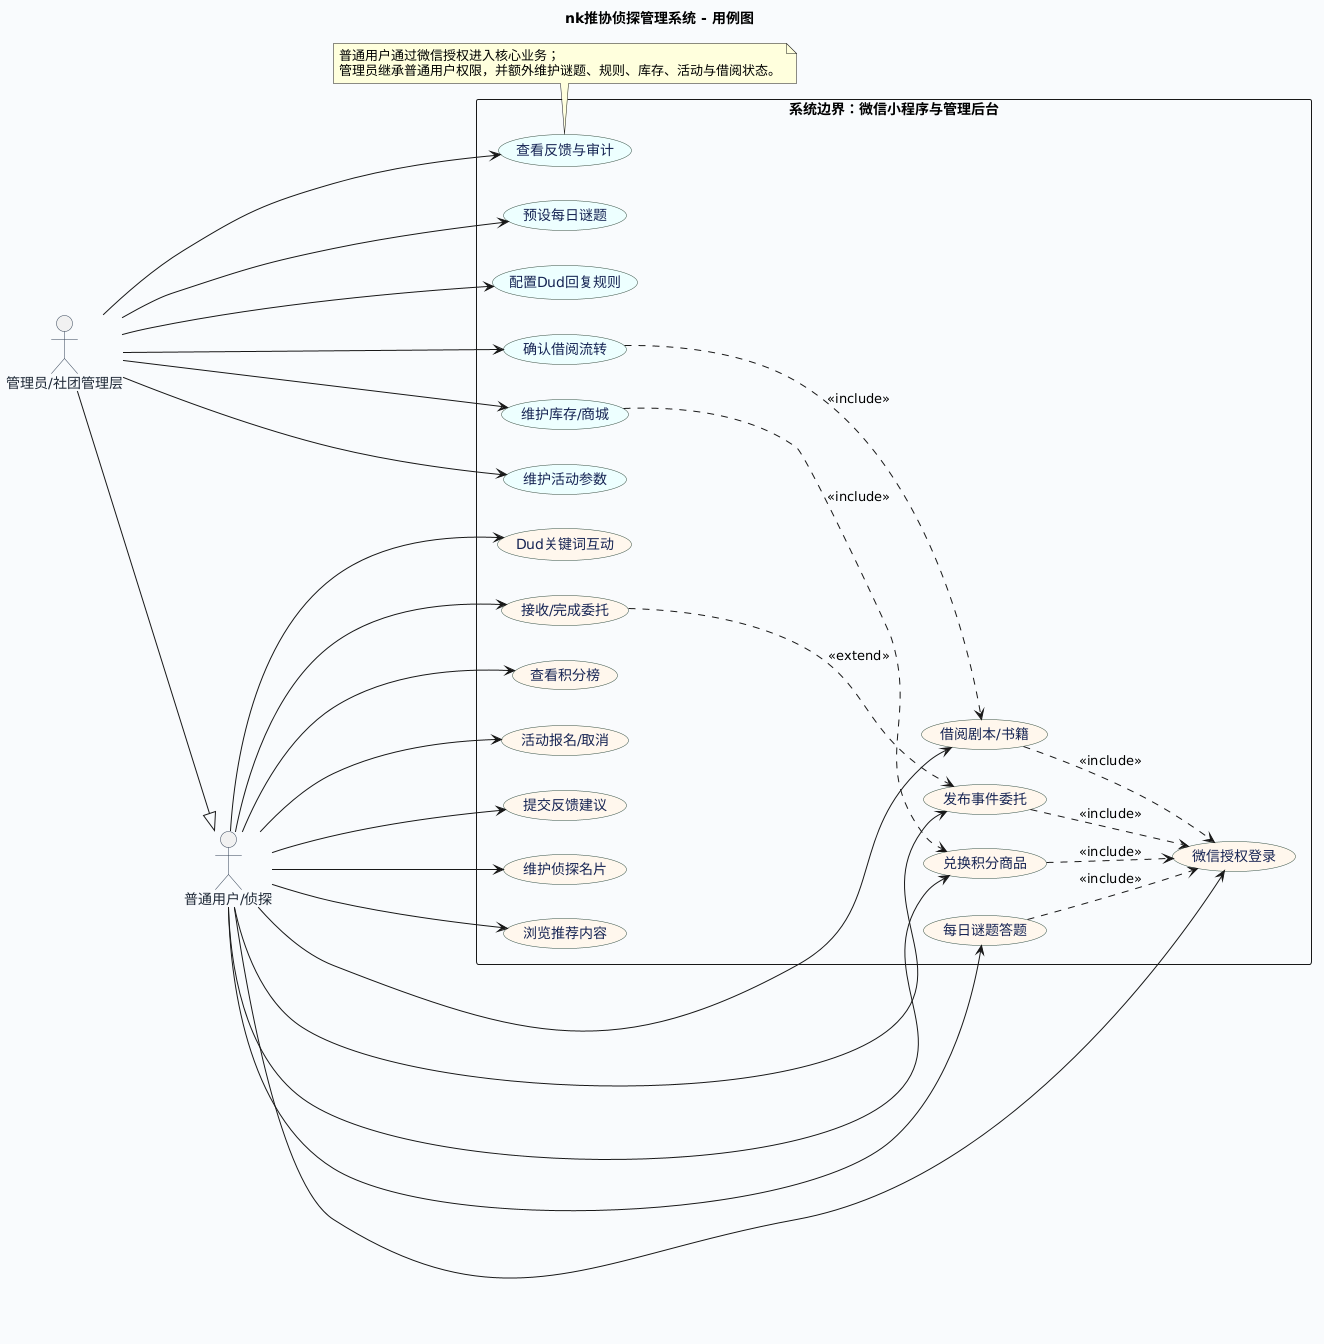
\includegraphics[width=0.58\textwidth,keepaspectratio]{uml_output/use_case_diagram.png}
  \caption{系统用例图}
  \label{fig:use-case-diagram}
\end{figure}

\subsection{2. 类图（Class Diagram）}
图 \ref{fig:class-diagram} 展示了功能需求对应的主要业务对象，包括用户、管理员、每日谜题、答题记录、积分账户、活动、物资、借阅记录、Dud回复规则、事件委托、反馈建议和推荐内容。后续需求描述均以这些对象及其关系为基础。
\begin{figure}[H]
  \centering
  
\includegraphics[width=0.68\textwidth,keepaspectratio]{uml_output/class_diagram.png}
  \caption{系统概念类图}
  \label{fig:class-diagram}
\end{figure}

\subsection{3. 顺序图（Sequence Diagram）}

\subsubsection*{活动报名顺序图}

图 \ref{fig:seq-activity} 展示了用户报名活动的完整交互流程，整体可分为“加载活动列表”和“提交活动报名”两个阶段。用户进入活动页面后，页面调用前端请求封装，由 \texttt{activity} 云函数查询 \texttt{activities} 集合并返回未取消的活动列表，前端据此完成列表渲染。用户点击报名后，页面首先检查活动剩余名额和报名理由，再通过云函数进行后端校验，包括登录状态、活动是否存在、是否重复报名以及活动容量限制等。若校验失败，系统直接返回失败原因并提示用户；若超过最晚取消时间，则返回二次确认标识，由前端弹窗确认后再次提交。校验通过后，云函数更新活动已报名人数，并新增 \texttt{activity\_registrations} 报名记录，最后返回报名成功，前端关闭弹窗并刷新活动列表与用户的活动记录。

\begin{figure}[H]
  \centering
  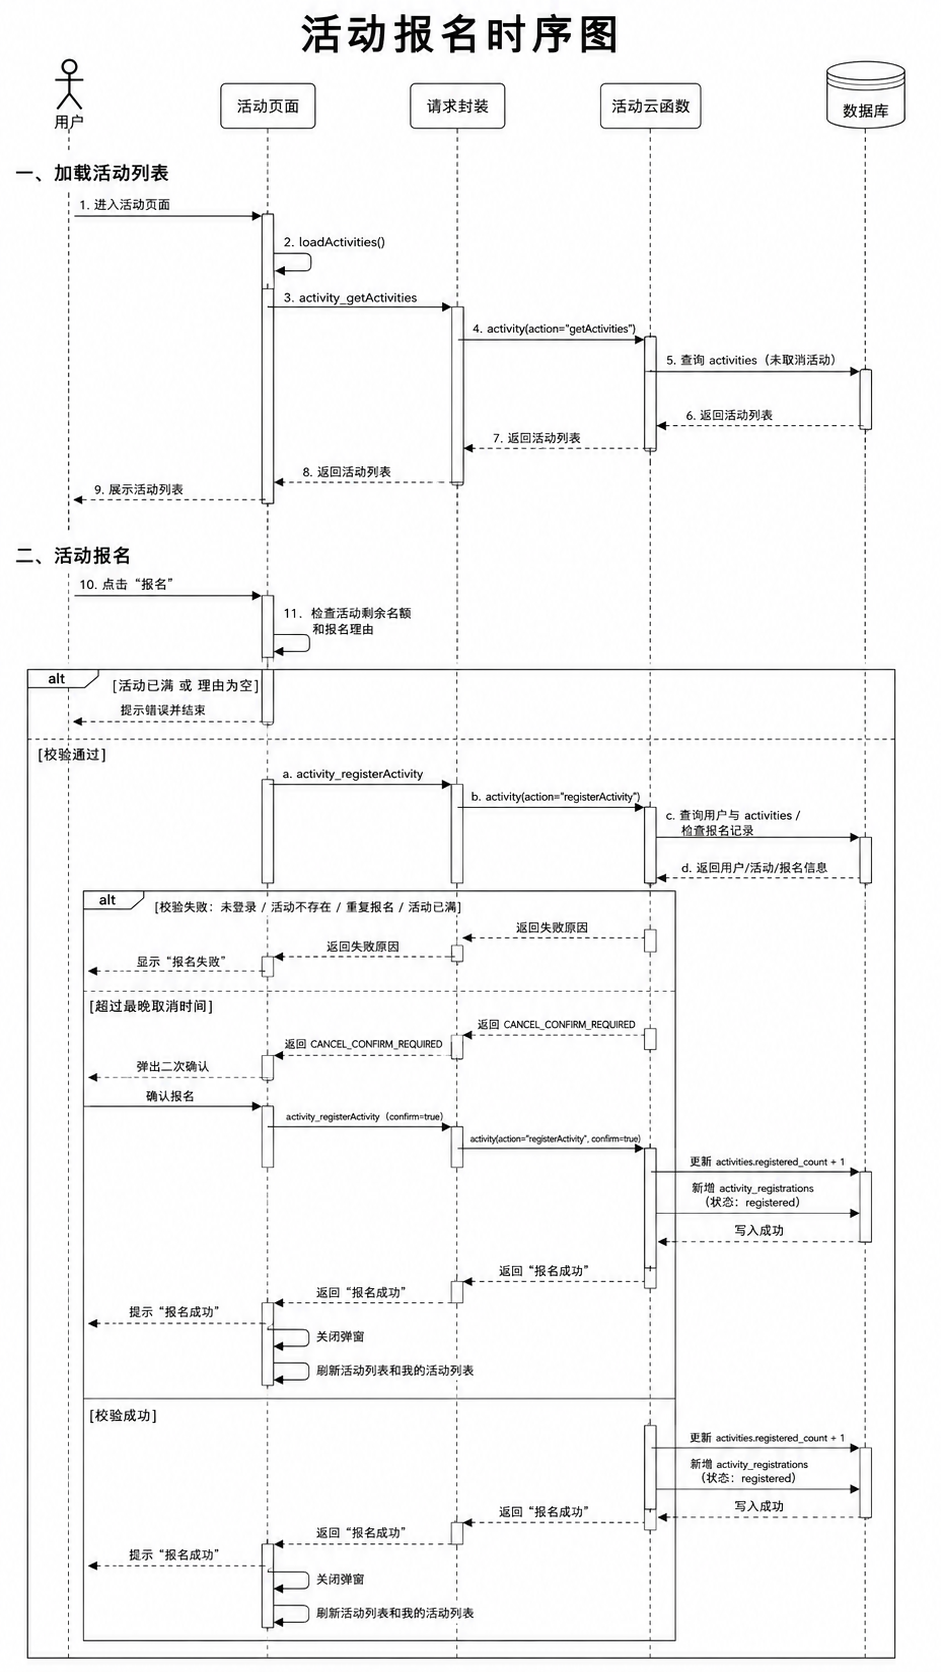
\includegraphics[width=0.70\textwidth,height=0.78\textheight,keepaspectratio]{activity_sequence_graph.png}
  \caption{活动报名顺序图}
  \label{fig:seq-activity}
\end{figure}

\subsubsection*{物资借阅顺序图}

图 \ref{fig:seq-borrow} 展示了用户借阅物资的完整交互流程，整体可分为“加载可借物品”和“申请借阅”两个阶段。用户进入借阅页面后，页面调用 \texttt{borrow} 云函数查询 \texttt{inventory\_items} 集合，返回当前可借物品列表并展示。用户提交申请时，前端先检查物品状态和借阅理由，后端随后再次校验登录状态、物品是否存在以及状态是否为 \texttt{available}。若物品不可借、理由为空或后端校验失败，系统返回失败原因并在页面提示；校验通过后，云函数新增 \texttt{borrow\_applications} 申请记录、写入 \texttt{borrow\_records} 借阅记录，并将物品状态更新为 \texttt{in\_transit}。流程结束后，前端关闭申请弹窗，刷新物品列表和“我的借阅”记录，保证页面状态与数据库状态一致。

\begin{figure}[H]
  \centering
  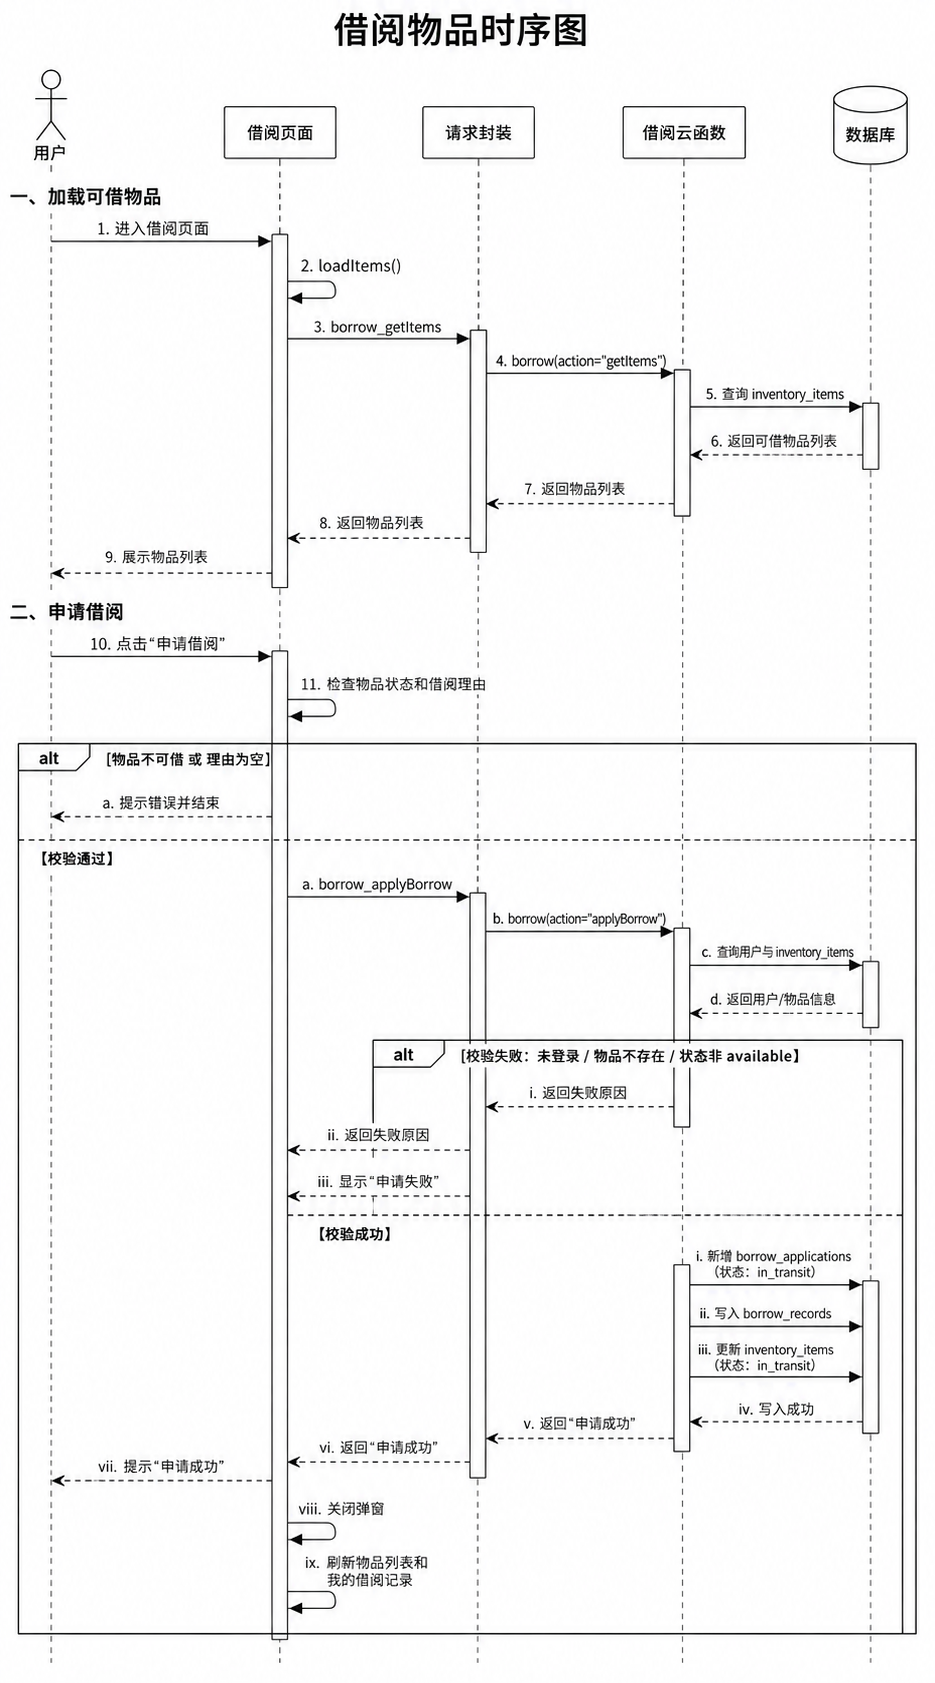
\includegraphics[width=0.70\textwidth,height=0.78\textheight,keepaspectratio]{borrow_sequence_graph.png}
  \caption{物资借阅顺序图}
  \label{fig:seq-borrow}
\end{figure}

\subsection{4. 状态图、组件图或部署图（可选）}

\subsubsection*{系统组件图}

图 \ref{fig:component} 展示了系统的组件架构，包括微信小程序前端、前端服务层、工具模块、云函数服务层和云数据库五类核心组成部分。前端页面组件覆盖首页、物资借阅页、活动报名页、个人中心页和后台管理页等主要入口；前端服务层通过 \texttt{borrow.js}、\texttt{activity.js}、\texttt{user.js}、\texttt{points.js} 等文件封装业务请求；工具模块提供请求封装、认证、本地存储和格式化能力。云函数服务层按照业务域拆分为 \texttt{user}、\texttt{borrow}、\texttt{activity}、\texttt{points}、\texttt{admin} 等模块，并通过 \texttt{wx-server-sdk} 访问 \texttt{users}、\texttt{inventory\_items}、\texttt{borrow\_applications}、\texttt{borrow\_records}、\texttt{activities}、\texttt{activity\_registrations} 和 \texttt{points\_records} 等集合。该组件划分体现了页面展示、请求封装、业务处理和数据持久化之间的分层依赖关系。

\begin{figure}[H]
  \centering
  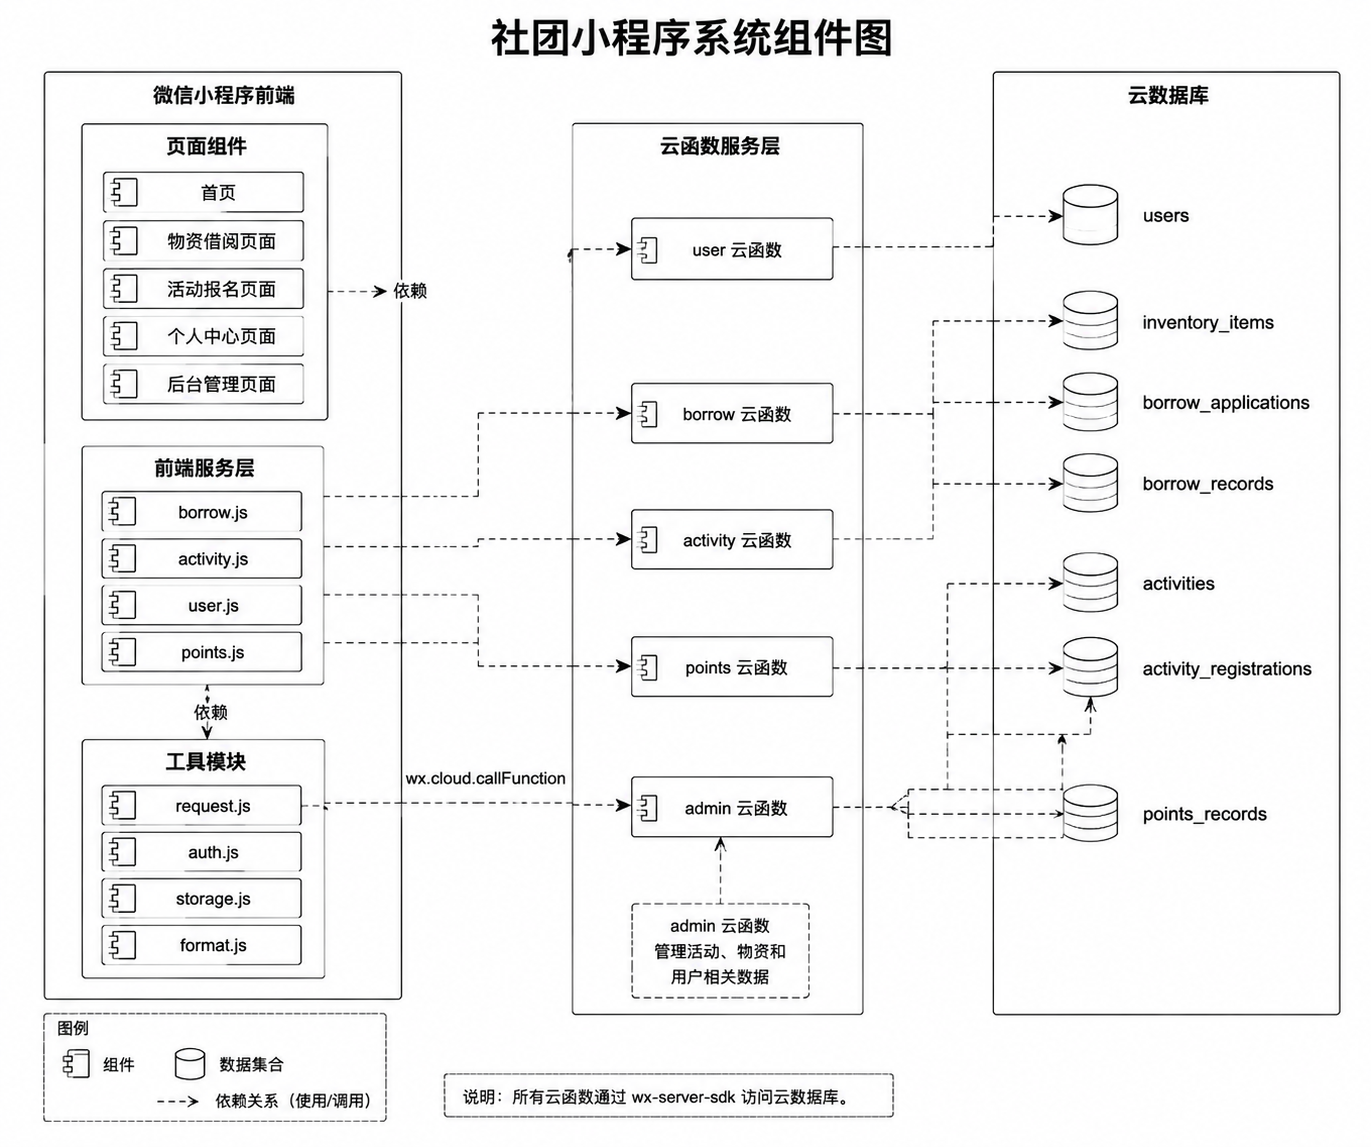
\includegraphics[width=0.90\textwidth,height=0.68\textheight,keepaspectratio]{system_zujian.png}
  \caption{系统组件图}
  \label{fig:component}
\end{figure}

\subsubsection*{系统部署图}

图 \ref{fig:deployment} 展示了系统的物理部署架构。用户通过移动设备上的微信客户端访问社团小程序前端，小程序运行环境负责页面渲染、事件处理、本地缓存和 \texttt{wx.cloud.callFunction} 调用。业务逻辑部署在微信云开发环境 \texttt{cloud1} 中，由 Node.js 云函数运行环境承载 \texttt{user}、\texttt{admin}、\texttt{borrow}、\texttt{exchange}、\texttt{activity}、\texttt{ranking}、\texttt{points} 等云函数。云函数进一步读写云数据库中的用户、物资、借阅、活动和积分相关集合；图片资源、小程序配置文件和默认封面图标等静态内容则由云存储或静态资源节点提供。该部署方式将客户端交互、云端业务计算、数据持久化和静态资源管理分离，降低了自建服务器的维护成本。

\begin{figure}[H]
  \centering
  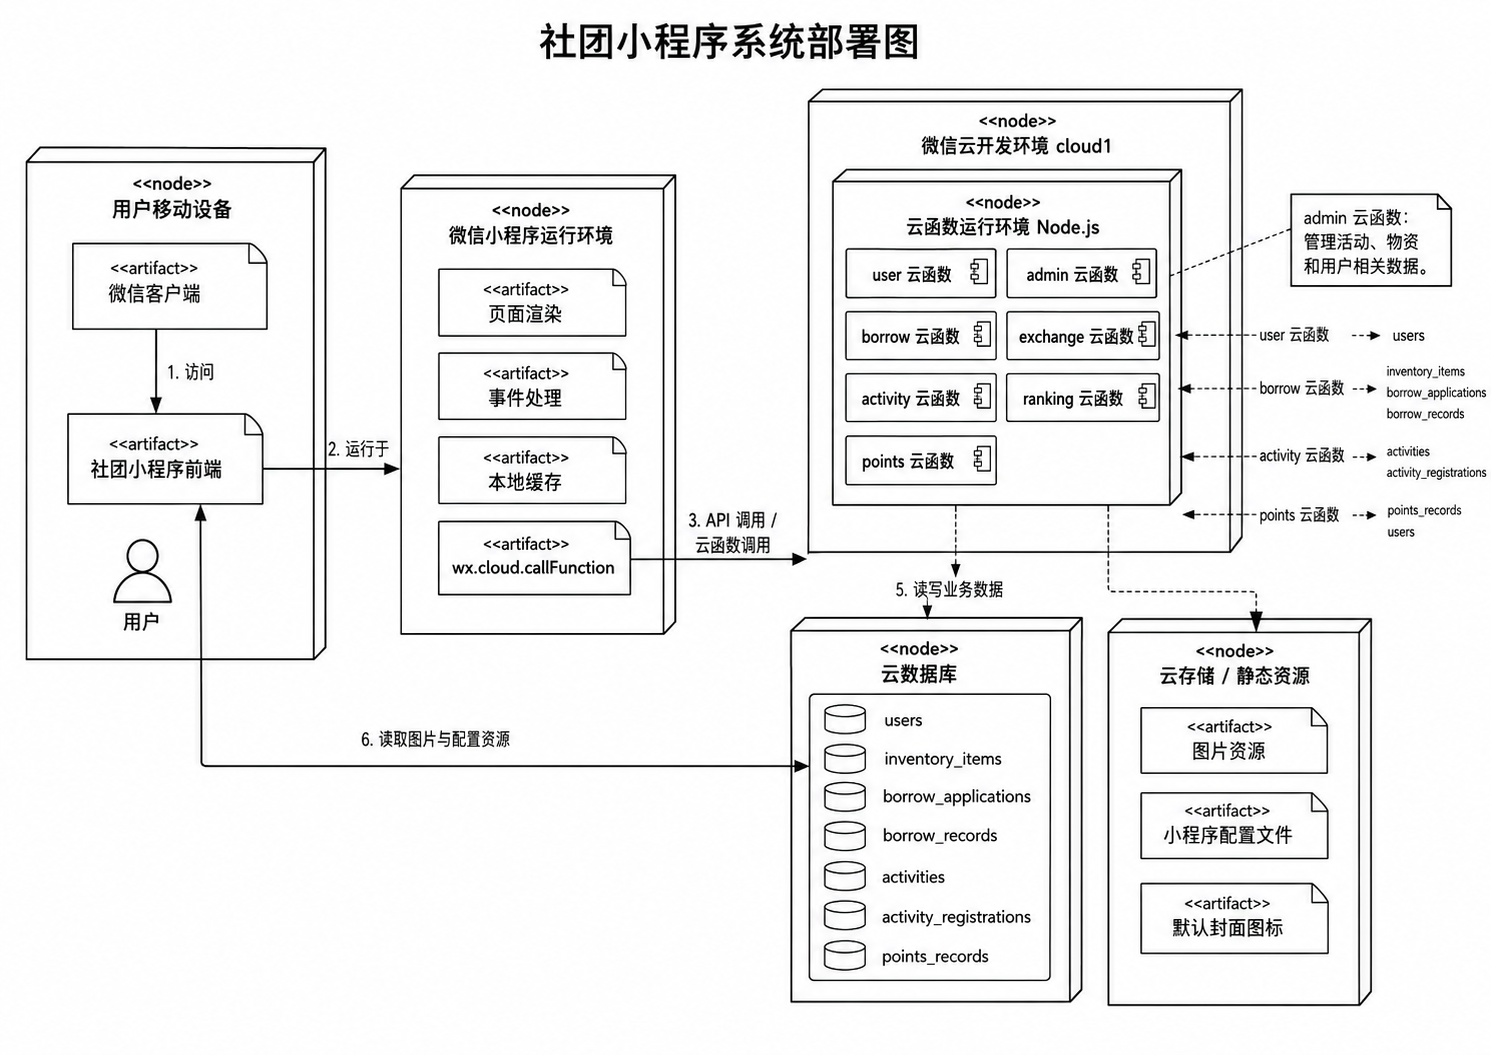
\includegraphics[width=0.90\textwidth,height=0.68\textheight,keepaspectratio]{system-managment.png}
  \caption{系统部署图}
  \label{fig:deployment}
\end{figure}

\section{四、数据库设计}

\subsection{1. 数据库 E-R 图}

本系统采用文档型 NoSQL 数据库，不存在传统关系型数据库中严格的表联接与外键约束，但各集合之间通过文档 ID 引用形成了逻辑上的实体关系。以下通过两张 E-R 图分别展示核心业务实体和支撑性实体的逻辑关联。

\subsubsection*{核心业务 E-R 图}

图 \ref{fig:er-core} 展示了用户、谜题、活动、物资借阅、兑换和事件委托六大业务域的实体及其关系。用户（\texttt{users}）是系统的中心实体，与各业务域的关联实体通过 \texttt{user\_id} 建立联系。

\begin{figure}[H]
  \centering
  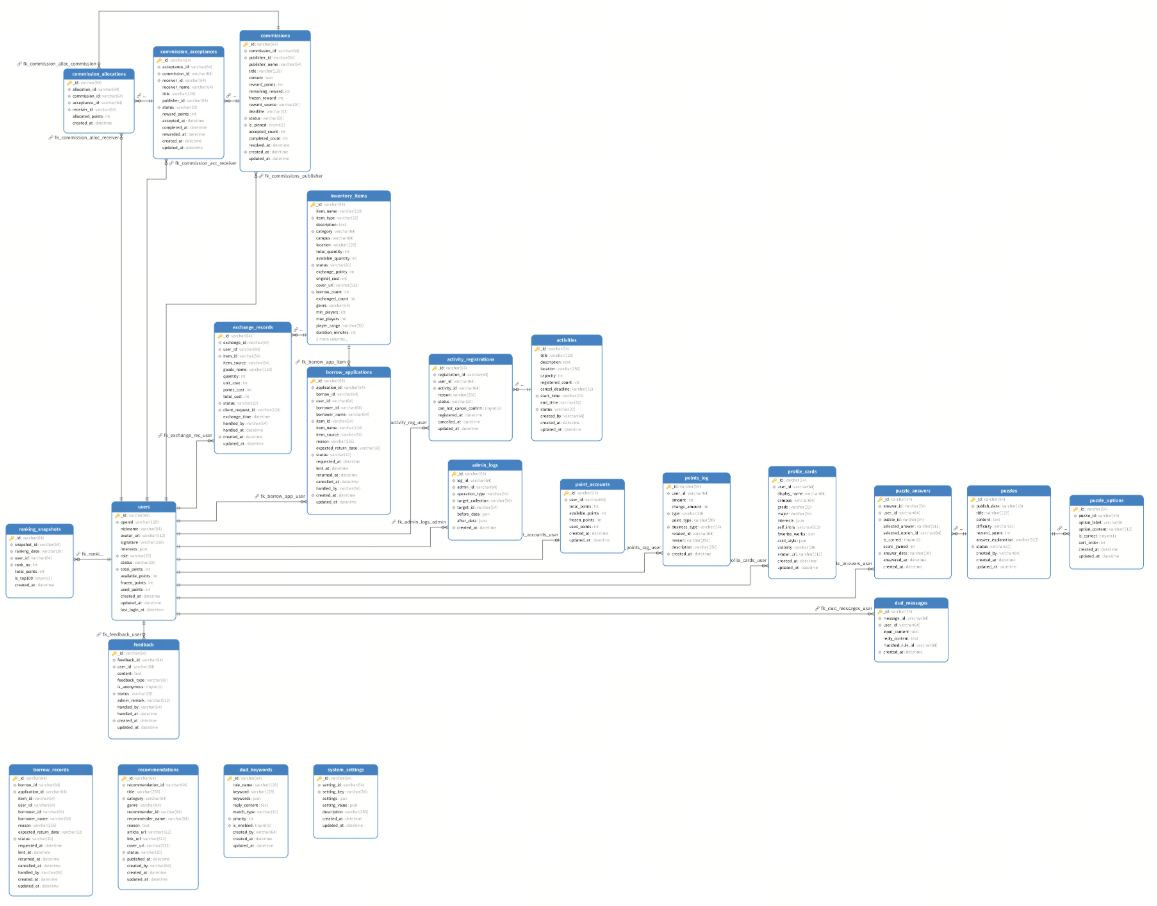
\includegraphics[width=\textwidth,keepaspectratio]{er_image.png}
  \caption{核心业务数据库 E-R 图}
  \label{fig:er-core}
\end{figure}

\subsubsection*{支撑性实体 E-R 图}

图 \ref{fig:er-support} 展示了 Dud 聊天、反馈留言、推荐内容、排行榜快照、系统设置和管理审计日志等支撑性实体。这些实体大多仅与用户存在单向关联，或为独立实体。

\begin{figure}[H]
  \centering
  \resizebox{0.75\textwidth}{!}{
    \begin{tikzpicture}[
        entity/.style={
            rectangle, draw=black, line width=0.7pt, fill=blue!7,
            minimum width=2.4cm, minimum height=0.7cm,
            font=\footnotesize\bfseries, align=center, rounded corners=2pt,
            inner sep=4pt
          },
        assoc/.style={
            rectangle, draw=black, line width=0.5pt, fill=yellow!10,
            minimum width=2.4cm, minimum height=0.65cm,
            font=\footnotesize, align=center, rounded corners=2pt,
            inner sep=3pt
          },
        independent/.style={
            rectangle, draw=black!50, line width=0.5pt, fill=green!5,
            minimum width=2.4cm, minimum height=0.65cm,
            font=\footnotesize, align=center, rounded corners=2pt,
            inner sep=3pt
          },
        onetomany/.style={>=stealth, ->, thick, draw=blue!60!black},
        label/.style={font=\tiny\itshape, fill=white, inner sep=1pt},
      ]
      % Central user
      \node [entity, minimum width=2.8cm, minimum height=0.8cm, fill=blue!15] (users) at (0, 0) {\textbf{用户}\\(users)};

      % Left side: user-associated entities
      \node [assoc] (dudmsg) at (-5, 3) {Dud 消息\\(dud\_messages)};
      \node [assoc] (feedback) at (-5, 0) {反馈留言\\(feedback)};

      % Right side: independent entities
      \node [independent] (dudkw) at (5, 4) {Dud 关键词\\(dud\_keywords)};
      \node [independent] (rec) at (5, 1.5) {推荐内容\\(recommendations)};
      \node [independent] (rank) at (5, -1.5) {排行榜快照\\(ranking\_snapshots)};
      \node [independent] (settings) at (5, -4) {系统设置\\(system\_settings)};
      \node [independent] (adminlog) at (0, -4) {管理日志\\(admin\_logs)};

      % Relationships
      \draw [onetomany] (users) -- (dudmsg) node [label, midway, left] {1 : N};
      \draw [onetomany] (users) -- (feedback) node [label, midway, above] {1 : N};

      % Group boxes
      \draw [draw=gray!40, dashed, rounded corners=6pt] (-7, -2) rectangle (-2.5, 5);
      \node [font=\tiny\color{gray}] at (-4.75, 5.3) {用户关联实体};

      \draw [draw=gray!40, dashed, rounded corners=6pt] (2.5, -5.5) rectangle (7.5, 6);
      \node [font=\tiny\color{gray}] at (5, 6.3) {独立实体};

      \draw [draw=gray!40, dashed, rounded corners=6pt] (-3, -6) rectangle (3, -3);
      \node [font=\tiny\color{gray}] at (0, -2.7) {审计实体};
    \end{tikzpicture}
  }
  \caption{支撑性实体 E-R 图}
  \label{fig:er-support}
\end{figure}

\textbf{实体关系说明。} 核心业务图中，用户（\texttt{users}）是整个系统的中心枢纽，与个人名片和积分账户保持一对一关系，与积分流水保持一对多关系。谜题（\texttt{puzzles}）拥有多个选项，用户通过答题记录与谜题建立多对多联系。活动与用户之间通过报名记录关联。库存物资同时服务于借阅和兑换两条业务线：用户通过借阅申请与物资建立借阅关系（另有借阅记录作为冗余视图），通过兑换记录与物资建立兑换关系。事件委托涉及三方关系——发布者创建委托，领取者通过领取记录参与委托，奖励通过分配记录从委托流转至领取者。支撑性实体中，Dud 消息和反馈留言直接关联用户；Dud 关键词、推荐内容、排行榜快照和系统设置为独立实体；管理日志记录管理员的操作审计信息。所有实体间的关联均通过文档 ID（\texttt{user\_id}、\texttt{puzzle\_id}、\texttt{item\_id}、\texttt{commission\_id} 等）实现逻辑引用。

\subsection{2. 主要数据表设计}

各集合的主键为云数据库自动生成的 \texttt{\_id}，业务主键另行定义为 \texttt{*\_id} 字符串字段。时间戳字段统一使用 \texttt{db.serverDate()} 写入。以下按业务域组织核心集合的字段说明。

\subsubsection*{2.1 用户与积分域}

\begin{table}[H]
  \centering
  \caption{用户与积分域核心字段}
  \label{tab:schema-user}
  \scriptsize
  \resizebox{\textwidth}{!}{\begin{tabular}{p{2.8cm} p{3.2cm} p{2.2cm} p{5.5cm}}
      \toprule
      \textbf{集合}                               & \textbf{关键字段}                                                                                      & \textbf{类型/约束} & \textbf{说明}                                                                                                         \\
      \midrule
      \multirow{7}{*}{\texttt{users}}           & \texttt{openid}                                                                                    & String, 唯一     & 微信 OpenID，自然唯一键，由微信服务端注入                                                                                            \\
                                                & \texttt{nickname}, \texttt{avatar\_url}, \texttt{signature}                                        & String         & 用户展示信息                                                                                                              \\
                                                & \texttt{interests}                                                                                 & Array          & 兴趣标签数组                                                                                                              \\
                                                & \texttt{role}                                                                                      & String         & \texttt{user | admin}，角色标识                                                                                          \\
                                                & \texttt{total\_points}, \texttt{available\_points}, \texttt{frozen\_points}, \texttt{used\_points} & Number         & 四维积分账户                                                                                                              \\
                                                & \texttt{created\_at}, \texttt{updated\_at}, \texttt{last\_login\_at}                               & ServerDate     & 服务端时间戳                                                                                                              \\
      \cmidrule{2-4}
      \multirow{3}{*}{\texttt{point\_accounts}} & \texttt{user\_id}                                                                                  & String         & 关联 users，与 users 积分字段双写同步                                                                                           \\
                                                & \texttt{total\_points}, \texttt{available\_points}, \texttt{frozen\_points}, \texttt{used\_points} & Number         & 独立积分查询入口，原子 inc 更新                                                                                                  \\
      \cmidrule{2-4}
      \multirow{4}{*}{\texttt{points\_log}}     & \texttt{user\_id}, \texttt{related\_id}                                                            & String         & 积分主体与关联业务 ID                                                                                                        \\
                                                & \texttt{amount} / \texttt{change\_amount}                                                          & Number         & 变动金额                                                                                                                \\
                                                & \texttt{type}                                                                                      & String         & \texttt{income\allowbreak\ |\allowbreak\ freeze\allowbreak\ |\allowbreak\ unfreeze\allowbreak\ |\allowbreak\ spend} \\
                                                & \texttt{point\_type}, \texttt{business\_type}, \texttt{reason}                                     & String         & 积分维度、业务来源、变动原因                                                                                                      \\
      \cmidrule{2-4}
      \multirow{4}{*}{\texttt{profile\_cards}}  & \texttt{user\_id}                                                                                  & String, 唯一     & 关联 users，一对一                                                                                                        \\
                                                & \texttt{display\_name}, \texttt{avatar\_url}                                                       & String         & 名片展示名称与头像                                                                                                           \\
                                                & \texttt{campus}, \texttt{grade}, \texttt{major}                                                    & String         & 校区、年级、专业                                                                                                            \\
                                                & \texttt{interests}, \texttt{favorite\_works}                                                       & Array          & 兴趣标签、喜爱作品列表                                                                                                         \\
                                                & \texttt{visibility}                                                                                & String         & \texttt{public | private}                                                                                           \\
      \bottomrule
    \end{tabular}}
\end{table}

\subsubsection*{2.2 谜题域}

\begin{table}[H]
  \centering
  \caption{谜题域核心字段}
  \label{tab:schema-puzzle}
  \scriptsize
  \resizebox{\textwidth}{!}{\begin{tabular}{p{2.8cm} p{3.2cm} p{2.2cm} p{5.5cm}}
      \toprule
      \textbf{集合}                               & \textbf{关键字段}                                                       & \textbf{类型/约束}  & \textbf{说明}                \\
      \midrule
      \multirow{5}{*}{\texttt{puzzles}}         & \texttt{puzzle\_id}                                                 & String          & 业务主键                       \\
                                                & \texttt{title}, \texttt{content}                                    & String          & 题目标题与正文                    \\
                                                & \texttt{publish\_date}                                              & String          & 发布日期，用于匹配当日题目              \\
                                                & \texttt{reward\_points}                                             & Number          & 答对奖励积分，默认 10               \\
                                                & \texttt{status}                                                     & String          & \texttt{published | draft} \\
      \cmidrule{2-4}
      \multirow{3}{*}{\texttt{puzzle\_options}} & \texttt{puzzle\_id}                                                 & String          & 所属谜题，一对多                   \\
                                                & \texttt{option\_label}, \texttt{option\_content}                    & String          & 选项标签（A/B/C/D）与文本           \\
                                                & \texttt{is\_correct}, \texttt{sort\_order}                          & Boolean, Number & 正确标识、排序序号                  \\
      \cmidrule{2-4}
      \multirow{3}{*}{\texttt{puzzle\_answers}} & \texttt{answer\_id}                                                 & String, \_id    & 稳定 \_id，幂等防重               \\
                                                & \texttt{user\_id}, \texttt{puzzle\_id}                              & String          & 关联用户与谜题                    \\
                                                & \texttt{selected\_answer}, \texttt{selected\_option\_id}            & String          & 所选答案内容与选项 ID               \\
                                                & \texttt{is\_correct}, \texttt{score\_gained}, \texttt{answer\_date} & Mixed           & 判定、得分、答题日期                 \\
      \bottomrule
    \end{tabular}}
\end{table}

\subsubsection*{2.3 物资、借阅与兑换域}

\begin{table}[H]
  \centering
  \caption{物资与流转域核心字段}
  \label{tab:schema-inventory}
  \scriptsize
  \resizebox{\textwidth}{!}{\begin{tabular}{p{2.8cm} p{3.2cm} p{2.2cm} p{5.5cm}}
      \toprule
      \textbf{集合}                                    & \textbf{关键字段}                                                & \textbf{类型/约束}  & \textbf{说明}                                                                                                                    \\
      \midrule
      \multirow{5}{*}{\texttt{inventory\_items}}     & \texttt{item\_id}, \texttt{item\_name}                       & String          & 业务主键与名称                                                                                                                        \\
                                                     & \texttt{item\_type}                                          & String          & 品类：\texttt{book\allowbreak\ |\allowbreak\ script\allowbreak\ |\allowbreak\ supplies\allowbreak\ |\allowbreak\ exchange\_goods} \\
                                                     & \texttt{total\_quantity}, \texttt{available\_quantity}       & Number          & 总数量、可用数量，原子 inc 更新                                                                                                             \\
                                                     & \texttt{status}                                              & String          & 见物资状态图（\ref{fig:state-inventory}）                                                                                              \\
                                                     & \texttt{genre, min\_players, \dots}                          & Mixed           & 剧本杀/商品特有字段（见图注）                                                                                                                \\
      \cmidrule{2-4}
      \multirow{4}{*}{\texttt{borrow\_applications}} & \texttt{application\_id} / \texttt{borrow\_id}               & String          & 业务主键                                                                                                                           \\
                                                     & \texttt{item\_id}, \texttt{user\_id}                         & String          & 关联物资与借阅人                                                                                                                       \\
                                                     & \texttt{reason}, \texttt{expected\_return\_date}             & String          & 借阅理由、预计归还日期                                                                                                                    \\
                                                     & \texttt{status}                                              & String          & 见借阅状态图（\ref{fig:state-borrow}）                                                                                                 \\
      \cmidrule{2-4}
      \texttt{borrow\_records}                       & \multicolumn{2}{l}{字段结构与 \texttt{borrow\_applications} 一致}   & 借阅记录冗余视图，便于统一查询                                                                                                                                  \\
      \cmidrule{2-4}
      \multirow{3}{*}{\texttt{exchange\_records}}    & \texttt{exchange\_id}, \texttt{user\_id}                     & String          & 业务主键、关联用户                                                                                                                      \\
                                                     & \texttt{goods\_id} / \texttt{item\_id}, \texttt{goods\_name} & String          & 关联商品                                                                                                                           \\
                                                     & \texttt{cost}, \texttt{status}                               & Number, String  & 消耗积分；\texttt{pending\allowbreak\ |\allowbreak\ completed\allowbreak\ |\allowbreak\ cancelled}                                  \\
      \bottomrule
    \end{tabular}}
\end{table}

\vspace{-0.5cm}
\begin{itemize}[nosep, leftmargin=*, font=\footnotesize]
  \item \textbf{剧本杀特有字段：} \texttt{genre}（题材）、\texttt{min\_players} / \texttt{max\_players}（人数）、\texttt{duration\_minutes}（时长）、\texttt{difficulty}（难度）
  \item \textbf{兑换商品特有字段：} \texttt{cost}（所需积分）、\texttt{original\_cost}（原价）、\texttt{exchange\_count}（兑换次数）
\end{itemize}

\subsubsection*{2.4 委托域}

\begin{table}[H]
  \centering
  \caption{委托域核心字段}
  \label{tab:schema-commission}
  \scriptsize
  \setlength{\tabcolsep}{4pt}
  \renewcommand{\arraystretch}{1.18}
  \begin{tabularx}{\textwidth}{>{\raggedright\arraybackslash}p{3.0cm} >{\raggedright\arraybackslash}p{4.1cm} >{\raggedright\arraybackslash}p{1.5cm} >{\raggedright\arraybackslash}X}
      \toprule
      \textbf{集合}                                       & \textbf{关键字段}                                                                                               & \textbf{类型} & \textbf{说明}                                                                                                                        \\
      \midrule
      \multirow{5}{3.0cm}{\centering\ttfamily commissions} & \texttt{commission\_id}, \texttt{publisher\_id}                                                             & String      & 业务主键与发布者                                                                                                                           \\
                                                        & \texttt{reward\_points}, \texttt{remaining\_reward}, \linebreak \texttt{frozen\_reward}                     & Number      & 总奖励、剩余、已冻结积分                                                                                                                       \\
                                                        & \texttt{reward\_source}                                                                                     & String      & \texttt{publisher | official}，决定积分来源                                                                                               \\
                                                        & \texttt{deadline}, \texttt{is\_pinned}                                                                      & Mixed       & 截止时间、是否置顶                                                                                                                          \\
                                                        & \texttt{status}                                                                                             & String      & 见委托状态图（\ref{fig:state-commission}）                                                                                                 \\
      \cmidrule{2-4}
      \multirow{3}{3.0cm}{\centering\ttfamily commission\_\\acceptances} & \texttt{acceptance\_id}                                                                                     & String      & 稳定 \_id 幂等，格式 \texttt{ca\_\{cid\}\_\{uid\}}                                                                                        \\
                                                        & \texttt{commission\_id}, \texttt{receiver\_id}, \linebreak \texttt{publisher\_id}                           & String      & 三方关联                                                                                                                               \\
                                                        & \texttt{status}                                                                                             & String      & \texttt{accepted\allowbreak\ |\allowbreak\ completed\allowbreak\ |\allowbreak\ rewarded}\linebreak\texttt{|\allowbreak\ withdrawn} \\
      \cmidrule{2-4}
      \multirow{2}{3.0cm}{\centering\ttfamily commission\_\\allocations} & \texttt{allocation\_id}, \texttt{commission\_id}, \linebreak \texttt{acceptance\_id}, \texttt{receiver\_id} & String      & 分配记录主键与三方关联                                                                                                                        \\
                                                        & \texttt{allocated\_points}                                                                                  & Number      & 本次分配积分数额                                                                                                                           \\
      \bottomrule
    \end{tabularx}
\end{table}

\subsubsection*{2.5 活动与其他支撑实体}

\begin{table}[H]
  \centering
  \caption{活动与其他实体核心字段}
  \label{tab:schema-other}
  \scriptsize
  \resizebox{\textwidth}{!}{\begin{tabular}{p{2.6cm} p{4cm} p{2cm} p{5.1cm}}
      \toprule
      \textbf{集合}                                         & \textbf{关键字段}                                                                                                     & \textbf{类型}  & \textbf{说明}                                                                                                             \\
      \midrule
      \multirow{4}{*}{\texttt{activities}}                & \texttt{activity\_id}, \texttt{title}                                                                             & String       & 业务主键与标题                                                                                                                 \\
                                                          & \texttt{capacity}, \texttt{registered\_count}                                                                     & Number       & 容量与已报名人数                                                                                                                \\
                                                          & \texttt{deadline}, \texttt{start\_time}, \linebreak \texttt{end\_time}                                            & DateTime     & 时间窗口                                                                                                                    \\
                                                          & \texttt{status}                                                                                                   & String       & \texttt{registering\allowbreak\ |\allowbreak\ full\allowbreak\ |\allowbreak\ ended\allowbreak\ |\allowbreak\ cancelled} \\
      \cmidrule{2-4}
      \texttt{activity\_}\linebreak\texttt{registrations} & \texttt{registration\_id}, \texttt{activity\_id}, \linebreak \texttt{user\_id}, \texttt{reason}, \texttt{status}  & Mixed        & 报名记录，关联活动与用户                                                                                                            \\
      \cmidrule{2-4}
      \texttt{dud\_keywords}                              & \texttt{keyword}, \texttt{reply}, \texttt{match\_type}, \linebreak \texttt{priority}, \texttt{enabled}            & Mixed        & 关键词规则：exact/fuzzy 匹配、优先级、启停                                                                                             \\
      \cmidrule{2-4}
      \texttt{dud\_messages}                              & \texttt{user\_id}, \texttt{message}, \texttt{reply}                                                               & String       & 用户消息与系统回复                                                                                                               \\
      \cmidrule{2-4}
      \texttt{feedback}                                   & \texttt{user\_id}, \texttt{content}, \texttt{is\_anonymous}, \linebreak \texttt{status}, \texttt{handler\_note}   & Mixed        & 反馈内容、匿名标识、处理备注                                                                                                          \\
      \cmidrule{2-4}
      \texttt{recommendations}                            & \texttt{title}, \texttt{content}, \texttt{summary}, \linebreak \texttt{cover\_url}, \texttt{status}               & Mixed        & \texttt{published\allowbreak\ |\allowbreak\ draft\allowbreak\ |\allowbreak\ archived}                                   \\
      \cmidrule{2-4}
      \texttt{ranking\_snapshots}                         & \multicolumn{2}{l}{排行榜定期快照}                                                                                       & 预计算排序结果，加速查询                                                                                                                           \\
      \cmidrule{2-4}
      \texttt{system\_settings}                           & \multicolumn{2}{l}{键值对全局配置}                                                                                       & 系统级配置参数                                                                                                                                \\
      \cmidrule{2-4}
      \texttt{admin\_logs}                                & \texttt{admin\_id}, \texttt{action}, \linebreak \texttt{target\_collection}, \texttt{target\_id}, \texttt{detail} & Mixed        & 管理操作审计，客户端不可读                                                                                                           \\
      \bottomrule
    \end{tabular}}
\end{table}

\subsubsection*{2.6 关键状态流转}

系统中有四类核心实体具备状态字段，其流转规则如下：

\begin{figure}[H]
  \centering
  \begin{tikzpicture}[
      state/.style={rectangle, draw=black, rounded corners=3pt, minimum width=2.2cm, minimum height=0.7cm, font=\footnotesize, align=center, fill=blue!5},
      arrow/.style={>=stealth, ->, thick, font=\footnotesize},
      scale=0.85, transform shape,
    ]
    \node [state, fill=green!10] (avail) at (0, 0) {在库 (available)};
    \node [state, fill=yellow!10] (transit) at (4.5, 0) {传递中 (in\_transit)};
    \node [state, fill=orange!10] (borrowed) at (9, 2) {已借出 (borrowed)};
    \node [state, fill=blue!5] (returned) at (13.5, 2) {已归还 (returned)};
    \node [state, fill=gray!10] (bcancelled) at (9, -2) {已取消 (cancelled)};
    \draw [arrow] (avail) -- (transit) node [midway, above] {用户申请};
    \draw [arrow] (transit) -- (borrowed) node [midway, above, sloped] {管理员确认借出};
    \draw [arrow] (borrowed) -- (returned) node [midway, above] {管理员确认归还};
    \draw [arrow] (returned) to [bend right=50] (avail) node [pos=0.45, below, sloped] {恢复可借};
    \draw [arrow] (transit) -- (bcancelled) node [midway, right] {取消};
    \draw [arrow] (bcancelled) to [bend left=50] (avail) node [pos=0.45, below, sloped] {恢复可借};
  \end{tikzpicture}
  \caption{物资状态流转图（\texttt{inventory\_items.status}）}
  \label{fig:state-inventory}
\end{figure}

\begin{figure}[H]
  \centering
  \resizebox{0.95\textwidth}{!}{
    \begin{tikzpicture}[
        state/.style={rectangle, draw=black, rounded corners=3pt, minimum width=1.8cm, minimum height=0.6cm, font=\scriptsize, align=center, fill=blue!5},
        estate/.style={rectangle, draw=black, rounded corners=3pt, minimum width=1.8cm, minimum height=0.6cm, font=\scriptsize, align=center, fill=yellow!10},
        arrow/.style={>=stealth, ->, thick, font=\scriptsize},
      ]
      % Borrow application status
      \node [estate] (applying) at (0, 0) {申请中\\(applying)};
      \node [estate] (itransit) at (4.5, 0) {传递中\\(in\_transit)};
      \node [estate] (iborrowed) at (9, 1.3) {已借出\\(borrowed)};
      \node [estate] (ireturn) at (13.5, 1.3) {已归还\\(returned)};
      \node [estate] (icancel) at (9, -1.3) {已取消\\(cancelled)};
      \draw [arrow] (applying) -- (itransit);
      \draw [arrow] (itransit) -- (iborrowed);
      \draw [arrow] (iborrowed) -- (ireturn);
      \draw [arrow] (itransit) -- (icancel);
      \draw [arrow] (applying) -- (icancel);
    \end{tikzpicture}
  }
  \caption{借阅申请状态流转图（\texttt{borrow\_applications.status}）}
  \label{fig:state-borrow}
\end{figure}

\begin{figure}[H]
  \centering
  \begin{tikzpicture}[
      state/.style={rectangle, draw=black, rounded corners=3pt, minimum width=2.2cm, minimum height=0.7cm, font=\footnotesize, align=center, fill=blue!5},
      arrow/.style={>=stealth, ->, thick, font=\footnotesize},
      scale=0.85, transform shape,
    ]
    % Commission status (top row)
    \node [state, fill=green!10] (recruiting) at (0, 0) {招募中 (recruiting)};
    \node [state, fill=yellow!10] (progress) at (4.5, 0) {进行中 (in\_progress)};
    \node [state, fill=blue!10] (resolved) at (9, 0) {已解决 (resolved)};
    \node [state, fill=gray!10] (closed) at (13.5, 0) {已关闭 (closed)};
    \draw [arrow] (recruiting) -- (progress) node [midway, above] {有人领取};
    \draw [arrow] (progress) -- (resolved) node [midway, above] {奖励分配完毕};
    \draw [arrow] (recruiting) to [bend left=50] (closed) node [pos=0.4, above] {到期/手动关闭};
    \draw [arrow] (progress) to [bend left=50] (closed) node [pos=0.4, below] {到期/手动关闭};
    % Acceptance sub-status (bottom row)
    \node [state, fill=orange!10] (acc) at (0, -3.8) {已领取 (accepted)};
    \node [state, fill=orange!15] (comp) at (4.5, -3.8) {已完成 (completed)};
    \node [state, fill=orange!20] (rewarded) at (9, -3.8) {已发放 (rewarded)};
    \node [state, fill=gray!10] (withdrawn) at (13.5, -3.8) {已退回 (withdrawn)};
    \draw [arrow] (acc) -- (comp);
    \draw [arrow] (comp) -- (rewarded) node [midway, above] {发布者分配};
    \draw [arrow] (acc) -- (withdrawn);
    \node [font=\footnotesize\itshape, below=0.5cm of rewarded] {\texttt{commission\_acceptances.status}};
  \end{tikzpicture}
  \caption{委托与领取状态流转图}
  \label{fig:state-commission}
\end{figure}

\subsubsection*{2.7 数据库安全规则概要}

云数据库所有集合均配置自定义安全规则，核心原则为“客户端仅读、云函数全权写”。各集合的权限分级如下：

\begin{table}[H]
  \centering
  \caption{数据库安全规则分级}
  \label{tab:security-rules}
  \scriptsize
  \resizebox{\textwidth}{!}{\begin{tabular}{p{2.8cm} p{2.2cm} p{8.5cm}}
      \toprule
      \textbf{权限级别} & \textbf{涉及集合}                                                                               & \textbf{读权限规则}        \\
      \midrule
      全员可读          & \texttt{puzzles}, \texttt{puzzle\_options}, \texttt{activities}, \texttt{inventory\_items},                         \\& \texttt{commissions}, \texttt{commission\_allocations}, \texttt{dud\_keywords},\\& \texttt{recommendations}, \texttt{ranking\_snapshots}, \texttt{system\_settings},\\& \texttt{profile\_cards} & \texttt{read: true}（公开数据，无需认证） \\
      \midrule
      仅本人可读         & \texttt{users}, \texttt{point\_accounts}, \texttt{points\_log}, \texttt{puzzle\_answers},                           \\& \texttt{activity\_registrations}, \texttt{borrow\_applications}, \texttt{borrow\_records},\\& \texttt{exchange\_records}, \texttt{commission\_acceptances},\\& \texttt{dud\_messages}, \texttt{feedback} & \texttt{read:\allowbreak\ auth.openid\allowbreak\ ==\allowbreak\ doc.openid}\\& 或通过 \texttt{get()} 跨集合校验关联用户 \\
      \midrule
      全员不可读         & \texttt{admin\_logs}                                                                        & \texttt{read: false}  \\&（仅通过 admin 云函数间接访问） \\
      \midrule
      全部集合          & 上述全部                                                                                        & \texttt{write: false} \\&（禁止客户端直接写入） \\
      \bottomrule
    \end{tabular}}
\end{table}

安全规则通过 \texttt{get} 函数实现跨集合权限判断——例如 \texttt{point\_accounts} 的可读性取决于\\\texttt{get(`database.users.\$\{doc.user\_id\}').openid\allowbreak == auth.openid}，确保仅积分账户所属用户本人可读取。

\subsubsection*{2.8 集合总览}

各核心集合按其业务归属分类汇总如下：

\begin{table}[H]
  \centering
  \caption{数据库核心集合一览}
  \label{tab:collections}
  \scriptsize
  \resizebox{\textwidth}{!}{\begin{tabular}{p{2.5cm} p{1.4cm} p{4.2cm} p{5cm}}
      \toprule
      \textbf{集合名称}                                       & \textbf{业务域} & \textbf{主要关联键}                           & \textbf{核心存储内容}           \\
      \midrule
      \texttt{users}                                      & 用户           & \texttt{openid}（唯一）                      & 用户信息、四维积分、角色与状态           \\
      \texttt{profile\_cards}                             & 个人名片         & \texttt{user\_id}                        & 校区、年级、专业、兴趣、喜爱作品、可见性      \\
      \texttt{point\_accounts}                            & 积分           & \texttt{user\_id}                        & 四维积分双写备份，独立查询入口           \\
      \texttt{points\_log}                                & 积分           & \texttt{user\_id}                        & 积分变动流水，金额、类型、业务来源         \\
      \texttt{puzzles}                                    & 日常谜题         & 日期                                       & 题目正文、难度、奖励积分、答案解析         \\
      \texttt{puzzle\_options}                            & 日常谜题         & \texttt{puzzle\_id}                      & 每题四个选项，正确标识与排序            \\
      \texttt{puzzle\_answers}                            & 日常谜题         & \texttt{user\_id}, \texttt{puzzle\_id}   & 答题记录，稳定\_id幂等防重           \\
      \texttt{activities}                                 & 活动           & —                                        & 活动标题、容量、时间窗口、状态           \\
      \texttt{activity\_}\linebreak\texttt{registrations} & 活动           & \texttt{activity\_id}, \texttt{user\_id} & 报名记录，理由与状态                \\
      \texttt{inventory\_items}                           & 借阅/兑换        & —                                        & 统一库存，按 item\_type 区分品类与数量 \\
      \texttt{borrow\_}\linebreak\texttt{applications}    & 借阅           & \texttt{item\_id}, \texttt{user\_id}     & 借阅申请，全生命周期状态流转            \\
      \texttt{borrow\_records}                            & 借阅           & \texttt{item\_id}, \texttt{user\_id}     & 借阅记录冗余视图                  \\
      \texttt{exchange\_records}                          & 兑换           & \texttt{user\_id}, \texttt{goods\_id}    & 兑换记录，消耗积分与领取状态            \\
      \texttt{commissions}                                & 委托           & \texttt{publisher\_id}                   & 委托发布、奖励积分、冻结与分配           \\
      \texttt{commission\_}\linebreak\texttt{acceptances} & 委托           & \texttt{receiver\_id}                    & 委托领取记录，状态流转与奖励分配          \\
      \texttt{commission\_}\linebreak\texttt{allocations} & 委托           & \texttt{commission\_id}                  & 奖励分配明细，接收者与金额             \\
      \texttt{dud\_keywords}                              & Dud          & —                                        & 关键词规则，匹配模式与优先级            \\
      \texttt{dud\_messages}                              & Dud          & \texttt{user\_id}                        & 用户消息与系统回复                 \\
      \texttt{feedback}                                   & 反馈           & \texttt{user\_id}                        & 反馈内容、匿名标识、处理备注            \\
      \texttt{recommendations}                            & 推荐           & —                                        & 推荐内容、摘要、上下架状态             \\
      \texttt{ranking\_snapshots}                         & 排行榜          & —                                        & 排行榜定期快照，加速查询              \\
      \texttt{system\_settings}                           & 系统           & —                                        & 全局配置键值对                   \\
      \texttt{admin\_logs}                                & 审计           & \texttt{admin\_id}                       & 管理操作审计，目标集合与详情            \\
      \bottomrule
    \end{tabular}}
\end{table}

\section{五、其他内容}

\subsection{1. 安全性设计}

本系统从多个层面构建安全防护体系，覆盖身份认证、数据访问控制和业务防作弊等维度。

\textbf{身份认证与授权。} 系统完全依赖微信 OAuth 体系，用户身份通过微信 OpenID 唯一确定，不自行维护密码体系，消除了密码泄露和暴力破解的风险。云函数内部通过 \texttt{cloud.\allowbreak getWXContext().\allowbreak OPENID} 获取调用者身份，该值由微信服务端注入，客户端无法伪造。管理员权限基于 \texttt{users} 集合中的 \texttt{role} 字段进行判断，初始管理员通过云函数环境变量\\\texttt{BOOTSTRAP\_ADMIN\_OPENID} 配置，后续管理员由已有管理员在数据库层面手动维护，避免了权限提升漏洞。

\textbf{数据库安全规则。} 所有数据库集合均配置了自定义安全规则，遵循“客户端仅读、云函数全权写”的原则。具体策略为：公开数据（谜题、活动、库存物资、推荐内容、Dud 关键词、排行榜快照、系统设置等）全员可读；私有数据（用户信息、积分账户、答题记录、活动报名、借阅记录、兑换记录、反馈、聊天记录等）仅文档所属用户可读；管理日志集合对所有客户端（包括管理员）不可读，仅能通过云函数间接访问。所有客户端直接写入操作统一禁止（\texttt{write: false}），确保任何数据变更都必须经过云函数的业务逻辑校验。安全规则使用 \texttt{get} 函数进行跨集合权限判断（如积分账户的可读性取决于关联用户的 OpenID 是否匹配当前登录用户），从数据库引擎层面杜绝越权访问。

\textbf{业务层防作弊。} 答题防重复通过稳定 \texttt{\_id} 幂等写入实现：格式为\\
\texttt{pa\_\{userId\}\_\{puzzleId\}\_\{date\}} 的 \texttt{\_id} 在云数据库中具有唯一性约束，并发的重复提交会在数据库层面被拒绝，杜绝双倍加分。委托领取同样使用稳定 \_id 防重复。积分冻结与扣减操作均使用条件更新语句（如 \texttt{where\{available\_points:\allowbreak\ \_.gte(reward)\}}），在数据库层面进行原子校验，防止积分不足时执行扣减或积分凭空产生。

\textbf{敏感信息保护。} 用户的 OpenID 绝不暴露在前端代码或返回给客户端的响应中。积分流水、借阅历史、答题记录等个人隐私数据在安全规则层面严格限定为仅本人可读。反馈系统支持匿名提交，用户的反馈记录仅本人和管理员可见。

\subsection{2. 性能优化设计}

针对微信小程序的运行环境和用户使用场景，系统在多个层次实施了性能优化措施。

\textbf{前端分包加载。} 小程序采用分包策略，仅将首页、谜题、排行榜和个人中心四个 Tab 页面纳入主包，其余10个业务页面（活动、借阅、兑换、委托、Dud、反馈、推荐、积分明细、设置、管理后台）均配置为独立子包（\texttt{subpackages}），在用户首次访问时才按需加载。这一策略有效降低了小程序的首屏加载时间。

\textbf{数据缓存策略。} 前端为三类高频读取数据配置了带过期时间的本地缓存：排行榜数据缓存60秒（排行榜页面访问频繁但实时性要求不高），用户信息缓存30分钟（减少每次页面切换时的云函数调用），推荐内容缓存1小时（首页推荐内容变化频率低）。缓存过期后自动从云函数刷新，用户在缓存有效期内直接读取本地数据，既提升了响应速度也降低了云函数调用次数。

\textbf{请求层优化。} \texttt{utils/request.js} 对云函数调用进行了统一封装，支持可配置的超时时间（默认为10秒，Dud 聊天为15秒，上传操作为30秒）和自动重试机制（指数退避策略，间隔为1秒、2秒、4秒）。并发请求数限制为最多10个，避免在页面加载时瞬间发起过多请求导致带宽竞争。分页查询统一限制每页最多50条，避免单次查询返回过多数据。

\textbf{服务端性能考量。} 云函数运行在腾讯云的无服务器环境，天然支持按需自动扩容。积分操作使用 \texttt{db.command.inc} 进行原子递增而非先读后写，减少了网络往返次数并避免了并发冲突。排行榜通过定期生成快照（\texttt{ranking\_snapshots}）将复杂的聚合排序计算前移，查询时直接读取快照而无需对全量用户数据进行实时排序。

\subsection{3. 可扩展性设计}

系统在设计层面预留了多方向的扩展空间以适应社团运营需求的变化。

\textbf{物资类型的灵活扩展。} \texttt{inventory\_items} 集合通过 \texttt{item\_type} 字段区分品类（book、script、script\_murder、supplies、exchange\_goods），新增物资类型只需在云函数的类型过滤逻辑中增加对应的枚举值而无需修改数据表结构。剧本杀特有的 \texttt{genre}、\texttt{min\_players}、\texttt{max\_players}、\texttt{duration\_minutes}、\texttt{difficulty} 等字段对于普通书籍或物资则为空，实现了同一集合内不同品类属性的灵活共存。

\textbf{积分来源的可追溯扩展。} 积分流水的 \texttt{business\_type} 字段标识每笔积分的来源（daily\_puzzle、commission\_reward、official\_commission\_reward、exchange\_spend、commission\_freeze 等），新增积分获取/消耗途径时只需定义新的业务类型标识并在对应云函数中调用统一的 \texttt{addPointLog} 写流水，不影响现有的积分统计和排行榜逻辑。

\textbf{角色体系的扩展预留。} \texttt{users} 集合的 \texttt{role} 字段设计为字符串类型而非布尔标识，当前取值为 \texttt{user} 和 \texttt{admin}，未来可扩展为更细粒度的角色体系（如“物资管理员”“活动管理员”等），只需在权限校验逻辑中增加对应的角色判断分支。

\textbf{云函数独立部署。} 15个云函数各自独立部署，一个云函数的更新不影响其他云函数的运行。各模块通过数据库集合共享数据（而非云函数间直接调用），模块间耦合度低，便于团队分工开发和独立迭代。

\subsection{4. 异常处理机制}

系统在前后端均建立了完整的异常处理体系，确保各层级的错误能被妥善捕获和处理。

\textbf{前端异常处理。} 所有异步操作均使用 try-catch 包裹。工具层的 \texttt{request.js} 在云函数调用失败时自动进行最多两次重试（指数退避），重试耗尽后返回统一的错误格式 \texttt{\{success:\allowbreak\ false,\allowbreak\ error:\allowbreak\ message\}}，业务服务层根据该格式向上层传递错误信息。App 全局注册了 \texttt{onError} 和 \texttt{onUnhandledRejection} 钩子，捕获未处理的 JavaScript 异常和 Promise 拒绝，本地记录错误信息（类型、消息、调用栈截断至2000字符、发生的页面路径和时间戳），供反馈页面或调试使用。页面路由错误通过 \texttt{onPageNotFound} 钩子兜底跳转至首页。

\textbf{后端异常处理与回滚。} 云函数中涉及多步数据更新的操作（如借阅申请、委托发布、奖励分配）均实现了手动回滚机制。以借阅申请为例：创建申请记录后若后续物资状态更新失败，系统自动将申请标记为“已取消”并将物资状态回滚至“在库”。委托发布的回滚同理：若 \texttt{commissions} 集合写入失败，已冻结的发布者积分将被自动解冻。奖励分配操作采用条件原子更新（领取记录必须为“已完成”状态、委托剩余奖励必须充足），任一条件不满足时拒绝操作并回滚已执行的步骤。

\textbf{集合缺失的优雅降级。} 云函数在访问数据库集合时统一捕获集合不存在的错误（错误码 -502005 或包含 “not exist” 的消息），此时返回空列表或跳过该集合操作而非抛出异常。这一设计使得云函数在新环境首次运行时即使数据库集合尚未创建，也能正常返回空结果而非报错，降低了部署和初始化的复杂度。

\textbf{幂等性保障。} 答题提交、委托领取等可能面临网络重试和用户重复点击的场景，系统通过稳定 \_id 实现操作幂等：并发重复请求中仅第一条能成功写入，后续请求因 \_id 冲突失败后自动查询已有记录并返回，用户感知为“已操作过”的友好提示而非异常错误。

\subsection{5. 日志与监控方案}

\textbf{管理操作审计。} 所有管理后台的增删改操作均写入 \texttt{admin\_logs} 集合，记录操作管理员 ID、操作类型、目标集合、目标文档 ID 和操作详情。该集合对所有客户端不可读，仅能通过云函数间接访问，确保审计日志的不可篡改性。

\textbf{积分流水追踪。} \texttt{points\_log} 集合完整记录了每笔积分的来源、去向、金额和业务类型，配合 \texttt{related\_id} 关联字段可追溯到具体的谜题、委托或兑换记录，为对账和争议处理提供数据基础。

\textbf{委托分配记录。} \texttt{commission\_allocations} 集合独立记录每笔委托奖励的分配细节（关联委托 ID、领取记录 ID、接收者 ID 和分配金额），与积分流水中的奖励记录形成双重追溯链。

\textbf{前端错误记录。} App 全局的 \texttt{recordError} 方法在内存中记录最近一次前端异常的类型、消息、截断后的调用栈和发生页面，该信息可通过反馈页面提交至后台，辅助开发者定位问题。

\textbf{后续优化方向。} 当前版本尚未集成专业的错误监控平台或性能分析工具（如微信官方的 WE 分析），建议后续版本接入以实现实时错误率告警、接口响应时间统计、用户行为漏斗分析等运营级监控能力。此外，云函数调用频率、数据库读写次数等云开发用量指标可通过腾讯云开发控制台进行基础监控。

\end{document}
